\documentclass[10pt,t]{beamer}


%\setbeamersize{text margin left=10pt,text margin right=10pt}
\usetheme{lehigh}


\usefonttheme{professionalfonts}
\usefonttheme{serif}


\pgfdeclarelayer{background}
\pgfdeclarelayer{foreground}
\pgfsetlayers{background,main,foreground}
%\usepackage{pgf,pgfarrows,pgfnodes,pgfautomata,pgfheaps,pgfshade}
%\usepackage{amsmath,amssymb,amsfonts,subfigure,pifont}
\usepackage{multirow,multicol}
%\usepackage{tabularx}
%\usepackage{booktabs}
\usepackage{colortbl}
\usepackage{algorithm,algpseudocode}
%\usepackage{etex}
\usepackage{fancyvrb,listings}

\definecolor{dkgreen}{rgb}{0,0.6,0}
\definecolor{gray}{rgb}{0.5,0.5,0.5}
\definecolor{mauve}{rgb}{0.58,0,0.82} 
\lstset{%
language=bash,                % the language of the code
%basicstyle=\footnotesize,           % the size of the fonts that are used for the code
basicstyle=\fontsize{4.5}{5.5}\selectfont\ttfamily,
showspaces=false,               % show spaces adding particular underscores
showstringspaces=false,         % underline spaces within strings
showtabs=false,                 % show tabs within strings adding particular underscores
%frame=single,                   % adds a frame around the code
%rulecolor=\color{black},        % if not set, the frame-color may be changed on line-breaks within not-black text (e.g. comments (green here))
tabsize=2,                      % sets default tabsize to 2 spaces
%captionpos=b,                   % sets the caption-position to bottom
breaklines=true,                % sets automatic line breaking
breakatwhitespace=false,        % sets if automatic breaks should only happen at whitespace
%title=\lstname,                   % show the filename of files included with \lstinputlisting;
% also try caption instead of title
keywordstyle=\color{blue},          % keyword style
commentstyle=\color{dkgreen},       % comment style
stringstyle=\color{mauve},         % string literal style
escapeinside={\%*}{*)},            % if you want to add LaTeX within your code
morekeywords={*,\dots,elif},              % if you want to add more keywords to the set
deletekeywords={\dots},              % if you want to delete keywords from the given language
%morecomment=[l]{//}
}
\lstset{%
language=csh,                % the language of the code
%basicstyle=\footnotesize,           % the size of the fonts that are used for the code
basicstyle=\fontsize{4.5}{5.5}\selectfont\ttfamily,
showspaces=false,               % show spaces adding particular underscores
showstringspaces=false,         % underline spaces within strings
showtabs=false,                 % show tabs within strings adding particular underscores
%frame=single,                   % adds a frame around the code
%rulecolor=\color{black},        % if not set, the frame-color may be changed on line-breaks within not-black text (e.g. comments (green here))
tabsize=2,                      % sets default tabsize to 2 spaces
captionpos=b,                   % sets the caption-position to bottom
breaklines=true,                % sets automatic line breaking
breakatwhitespace=false,        % sets if automatic breaks should only happen at whitespace
%title=\lstname,                   % show the filename of files included with \lstinputlisting;
% also try caption instead of title
keywordstyle=\color{blue},          % keyword style
commentstyle=\color{dkgreen},       % comment style
stringstyle=\color{mauve},         % string literal style
escapeinside={\%*}{*)},            % if you want to add LaTeX within your code
morekeywords={*,\dots,elif},              % if you want to add more keywords to the set
deletekeywords={\dots},              % if you want to delete keywords from the given language
%morecomment=[l]{//}
}
\lstdefinestyle{LINUX}
{
%    backgroundcolor=\color{black},
%    basicstyle=\tiny\ttfamily,
%    keywordsstyle=\color{blue},
%    morekeywords={Tutorials,BASH,scripts},
%    literate={>}{{\textcolor{blue}{>}}}1
%         {/}{{\textcolor{blue}{/}}}1
%         {./}{{\textcolor{black}{./ }}}1
%         {~}{{\textcolor{blue}{\textasciitilde}}}1,
}

\lstdefinestyle{customc}{
  belowcaptionskip=1\baselineskip,
  breaklines=true,
  xleftmargin=\parindent,
  language=C,
  showstringspaces=false,
  basicstyle=\scriptsize\ttfamily,
  keywordstyle=\bfseries\color{green!40!black},
  commentstyle=\upshape\color{red!90!white},
  identifierstyle=\color{blue},
  stringstyle=\color{orange},
}
\lstdefinelanguage{OmpFortran}[]{Fortran}{
   rulesepcolor=\color{black},
   %
   extendedchars=true,
   %
   morecomment=[l] [\bfseries\color{red!90!white}]{!\$omp},
   morecomment=[l] [\bfseries\color{red!90!white}]{c\$omp},
   morecomment=[l] [\bfseries\color{red!90!white}]{*\$omp},
   morecomment=[l] [\bfseries\color{red!90!white}]{!\$acc},
   morecomment=[l] [\bfseries\color{red!90!white}]{c\$acc},
   morecomment=[l] [\bfseries\color{red!90!white}]{*\$acc},
}[comments]

\lstdefinelanguage{OmpC}[]{OmpFortran}{
   rulesepcolor=\color{black},
   %
   extendedchars=true,
   %
   morecomment=[l] [\bfseries\color{red!90!white}]{\#pragma\ omp},
   morecomment=[l] [\bfseries\color{red!90!white}]{\#pragma\ acc},
}[comments]

\lstset{escapechar=@,style=customc}
\lstset{literate=%
   *{0}{{{\color{blue}0}}}1
    {1}{{{\color{blue}1}}}1
    {2}{{{\color{blue}2}}}1
    {3}{{{\color{blue}3}}}1
    {4}{{{\color{blue}4}}}1
    {5}{{{\color{blue}5}}}1
    {6}{{{\color{blue}6}}}1
    {7}{{{\color{blue}7}}}1
    {8}{{{\color{blue}8}}}1
    {9}{{{\color{blue}9}}}1
}

\algrenewcommand\algorithmicfunction{\textbf{program}}
\algblockdefx[Program]{Program}{EndProgram}[1]{\textbf{program} \textsc{#1}}[1]{\textbf{end program} \textsc{#1}}

\algloopdefx[doloop]{Do}[1]{\textbf{do} #1}
\algcblockdefx[doloop]{If}{Do}{EndDo}
[1]{\textbf{do} #1}{\textbf{end do}}




\usepackage{tikz}
\usetikzlibrary{shapes,arrows,matrix}
\usetikzlibrary{calc}
\pgfdeclarelayer{background}
\pgfdeclarelayer{foreground}
\pgfsetlayers{background,main,foreground}
%\usepackage[latin1]{inputenc}
\usepackage[english]{babel}
\usepackage{hyperref}
\usepackage[normalem]{ulem}
% \usepackage{movie15} 

                                                         
\usepackage{times}
\usepackage[T1]{fontenc}
\usepackage{graphicx}


\definecolor{DarkGreen}{rgb}{0.0,0.3,0.0}
\definecolor{Blue}{rgb}{0.0,0.0,0.8} 
\definecolor{dodgerblue}{rgb}{0.1,0.1,1.0}
\definecolor{indigo}{rgb}{0.41,0.1,0.0}
\definecolor{seagreen}{rgb}{0.1,1.0,0.1}
\DeclareSymbolFont{extraup}{U}{zavm}{m}{n}
%\DeclareMathSymbol{\vardiamond}{\mathalpha}{extraup}{87}
\newcommand{\cmark}{\ding{51}}
\newcommand{\xmark}{\ding{55}}
\newcommand{\smark}{\ding{77}}
\newcommand*\vardiamond{\textcolor{lubrown}{%
  \ensuremath{\blacklozenge}}}
\newcommand*\up{\textcolor{green}{%
  \ensuremath{\blacktriangle}}}
\newcommand*\down{\textcolor{red}{%
  \ensuremath{\blacktriangledown}}}
\newcommand*\const{\textcolor{darkgray}%
  {\textbf{--}}}
\newcommand*\enter{\tikz[baseline=-0.5ex] \draw[<-] (0,0) -| (0.5,0.1);}
\newcommand{\bftt}[1]{\textbf{\texttt{#1}}}
\newcommand{\lstfortran}[1]{\lstinline[language={[90]Fortran},basicstyle=\footnotesize\ttfamily]|#1|}
\newcommand{\Verblue}[1]{\Verb[formatcom=\color{blue},commandchars=\\\{\}]!#1!}
\newcommand{\Verbindigo}[1]{\Verb[formatcom=\color{indigo},commandchars=\\\{\}]!#1!}

\setbeamercolor{uppercol}{fg=white,bg=red!30!black}%
\setbeamercolor{lowercol}{fg=black,bg=red!15!white}%
\setbeamercolor{uppercol1}{fg=white,bg=blue!30!black}%
\setbeamercolor{lowercol1}{fg=black,bg=blue!15!white}%%
\setbeamercolor{uppercol2}{fg=white,bg=green!30!black}%
\setbeamercolor{lowercol2}{fg=black,bg=green!15!white}%
\newenvironment{colorblock}[4]
{
\setbeamercolor{upperblock}{fg=#1,bg=#2}
\setbeamercolor{lowerblock}{fg=#3,bg=#4}
\begin{beamerboxesrounded}[upper=upperblock,lower=lowerblock,shadow=false]}
{\end{beamerboxesrounded}}
\newenvironment{ablock}[0]
{
\begin{beamerboxesrounded}[upper=uppercol,lower=lowercol,shadow=false]}
{\end{beamerboxesrounded}}
\newenvironment{bblock}[0]
{
\begin{beamerboxesrounded}[upper=uppercol1,lower=lowercol1,shadow=false]}
{\end{beamerboxesrounded}}
\newenvironment{eblock}[0]
{
\begin{beamerboxesrounded}[upper=uppercol2,lower=lowercol2,shadow=false]}
{\end{beamerboxesrounded}}

% LOGOS
\pgfdeclareimage[height=0.55cm]{lucolor-logo}{LehighU_official-logo_Color.png}
\rplogo{\pgfuseimage{lucolor-logo}}
\pgfdeclareimage[height=0.55cm]{luwhite-logo}{LehighU_official-logo_White.png}
\tplogo{\pgfuseimage{luwhite-logo}}
% footer logo
%\pgfdeclareimage[width=0.3\paperwidth]{university-logo}{lulogo}
%\tllogo{\pgfuseimage{university-logo}}

%titlepage logo
%\titlegraphic{\includegraphics[scale=0.5]{lu}}

\beamertemplateballitem




\hypersetup{
  pdftitle={Modern Fortran}
  pdfauthor={Alexander B. Pacheco, User Services Consultant, Louisiana State University}
}

\title{Modern Fortran Programming II}


\author[Alex Pacheco]{\large{Alexander~B.~Pacheco}}
       
\institute{\href{http://researchcomputing.lehigh.edu}{LTS Research Computing}}

\date{\today}
     
\subject{Talks}
\keywords{Lehigh Research Computing Resources, Fortran Programming}
% This is only inserted into the PDF information catalog. Can be left
% out. 

% Delete this, if you do not want the table of contents to pop up at
% the beginning of each subsection:
\AtBeginSection[]
{
  \begingroup
  \setbeamertemplate{background canvas}[vertical shading][bottom=lubrown,top=lubrown]
  \setbeamertemplate{footline}[myfootline] 
  \setbeamertemplate{section page}[mysection]
  \frame[c]{
    \sectionpage
  }
  \endgroup
}

\titlegraphic{\includegraphics[scale=0.5]{lu}}

\begin{document}

\frame{\titlepage}

\begin{frame}{Outline}
  \tableofcontents
\end{frame}


\section{Arrays}
\begin{frame}{Arrays}
  \begin{itemize}
    \item Arrays (or matrices) hold a collection of different values at the same time.
    \item Individual elements are accessed by subscripting the array.
    \item A 10 element array is visualized as
    \item[]
      \begin{center}
        \begin{tabular}{|c|c|c|c|c|c|c|}
          \hline
          1 & 2 & 3 & $\cdots$ & 8 & 9 & 10 \\
          \hline
        \end{tabular}
      \end{center}
    \item[] while a 4x3 array as
    \item[]
      \begin{center}
        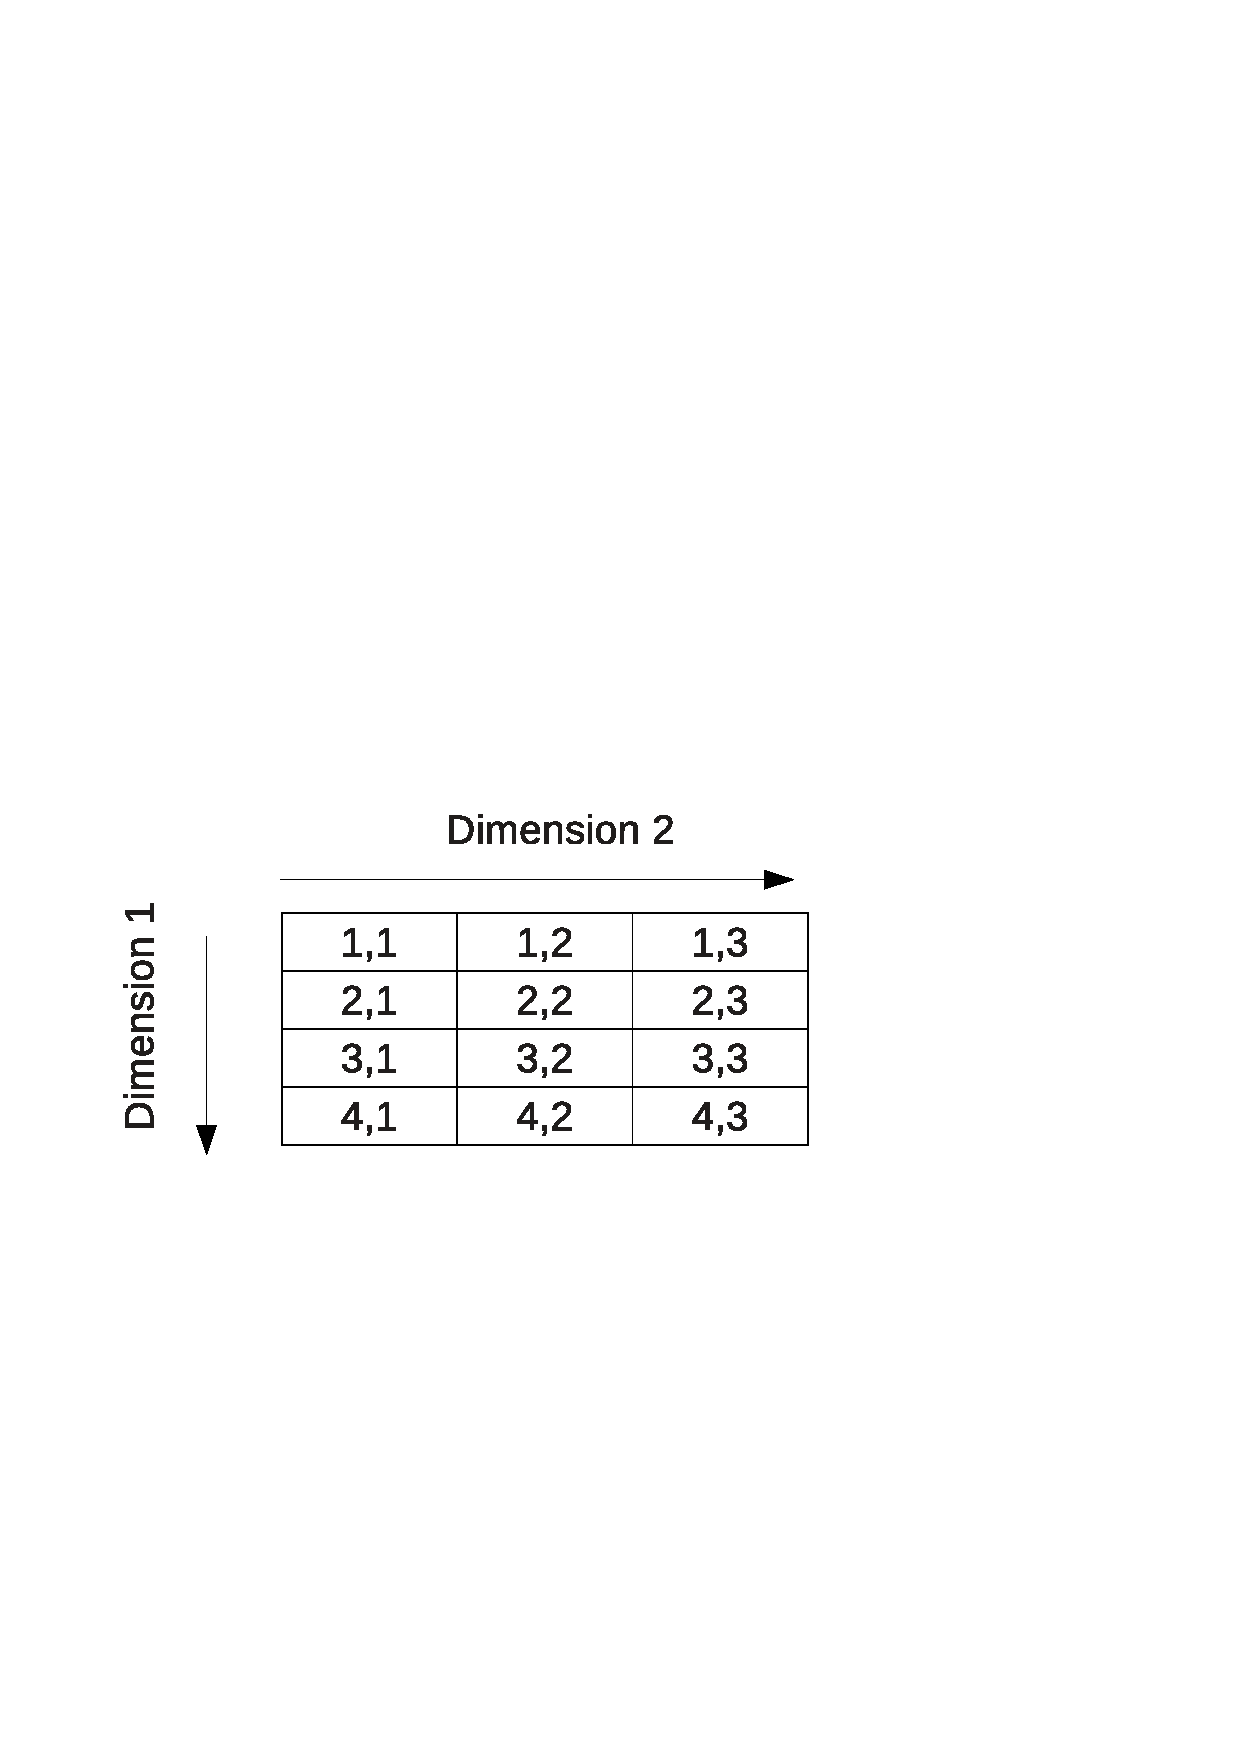
\includegraphics[width=4cm]{./graphics/array1}
      \end{center}
    \item Each array has a type and each element of holds a value of that type.
  \end{itemize}
\end{frame} 

\begin{frame}[fragile]{Array Declarations}
  \begin{itemize}
    \item The \lstfortran{dimension} attribute declares arrays.
    \item Usage: \lstfortran{dimension(lower\_bound:upper\_bound)}
    \item[] Lower bounds of one \lstfortran{(1:)} can be omitted
    \item Examples:
      \begin{lstlisting}[language={[90]Fortran}]
integer, dimension(1:106) :: atomic_number
real, dimension(3,0:5,-10:10) :: values
character(len=3),dimension(12) :: months
      \end{lstlisting}
    \item Alternative form for array declaration
      \begin{lstlisting}[language={[90]Fortran}]
integer :: days_per_week(7), months_per_year(12)
real :: grid(0:100,-100:0,-50:50)
complex :: psi(100,100)
      \end{lstlisting}
    \item Another alternative form which can be very confusing for readers
      \begin{lstlisting}[language={[90]Fortran}]
integer, dimension(7) :: days_per_week, months_per_year(12)
      \end{lstlisting}
  \end{itemize}
\end{frame}

\begin{frame}{Array Terminology}
  \begin{itemize}
    \item[] \lstfortran{real :: a(0:20), b(3,0:5,-10:10)}
  \end{itemize}
  \begin{description}
    \item[Rank:] Number of dimensions.
    \item[] {\lstfortran{a}} has rank 1 and {\lstfortran{b}} has rank 3
    \item[Bounds:] upper and lower limits of each dimension of the array.
    \item[] {\lstfortran{a}} has bounds 0:20 and {\lstfortran{b}} has bounds 1:3, 0:5 and -10:10
    \item[Extent:] Number of element in each dimension
    \item[] {\lstfortran{a}} has extent 21 and {\lstfortran{b}} has extents 3,6 and 21
    \item[Size:] Total number of elements.
    \item[] {\lstfortran{a}} has size 21 and {\lstfortran{b}} has 30
    \item[Shape:] The shape of an array is its rank and extent
    \item[] \lstfortran{a} has shape 21 and \lstfortran{b} has shape (3,6,21)
  \end{description}
  \begin{itemize}
    \item Arrays are conformable if they share a shape.
    \item The bounds do not have to be the same
    \item[] \lstfortran{c(4:6) = d(1:3)}
  \end{itemize}
\end{frame}

\begin{frame}[fragile]{Array Visualization}
  \begin{itemize}
    \item Define arrays \lstfortran{a,b,c} and \lstfortran{d} as follows
      \begin{lstlisting}[language={[90]Fortran}]
real,dimension(15) :: a
real,dimension(-4:0,0:2) :: b
real,dimension(5,3) :: c
real,dimension(4:8,2:4) :: d
      \end{lstlisting}
  \end{itemize}
  \begin{center}
    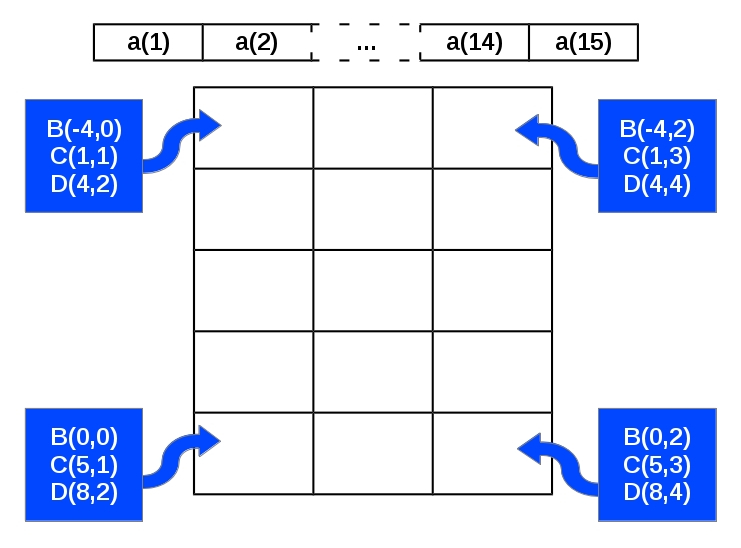
\includegraphics[width=5cm,clip=true]{./graphics/array2-3-1}
%    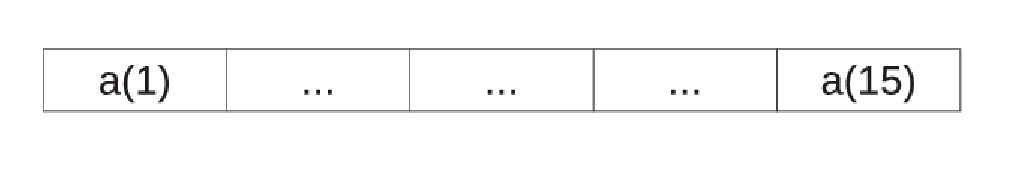
\includegraphics[width=4cm]{./graphics/array2}\\
%    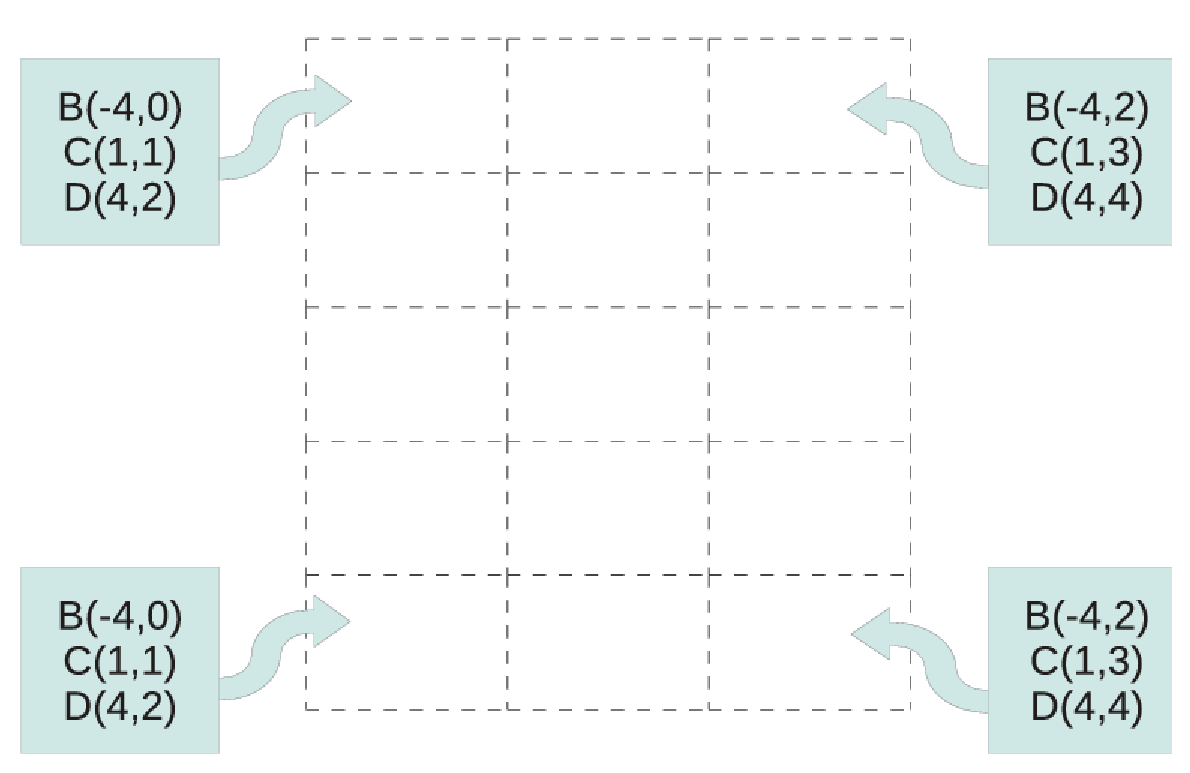
\includegraphics[width=4cm]{./graphics/array3}
  \end{center}
\end{frame}

\begin{frame}{Array Conformance}
  \begin{itemize}
    \item Array or sub-arrays must conform with all other objects in an expression
      \begin{enumerate}
        \item a scalar conforms to an array of any shape with the same value for every element
        \item[] \lstfortran{c = 1.0} is the same as \lstfortran{c(:,:) = 1.0}
        \item two array references must conform in their shape.
      \end{enumerate}
  \end{itemize}
  \begin{center}
    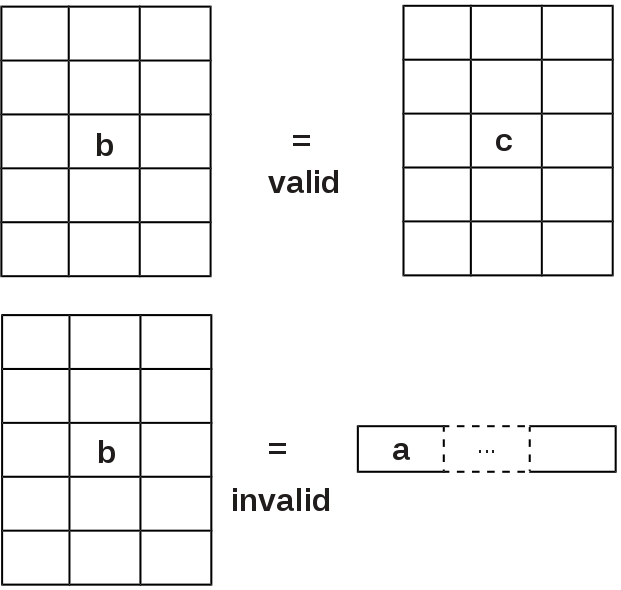
\includegraphics[width=4cm]{./graphics/array4}
  \end{center}
\end{frame}

\begin{frame}{Array Element Ordering}
  \begin{itemize}
    \item Fortran is a column major form i.e. elements are added to the columns seqeuntially. This ordering can be changed using the \lstfortran{reshape} intrinsic.
  \end{itemize}
  \begin{center}
    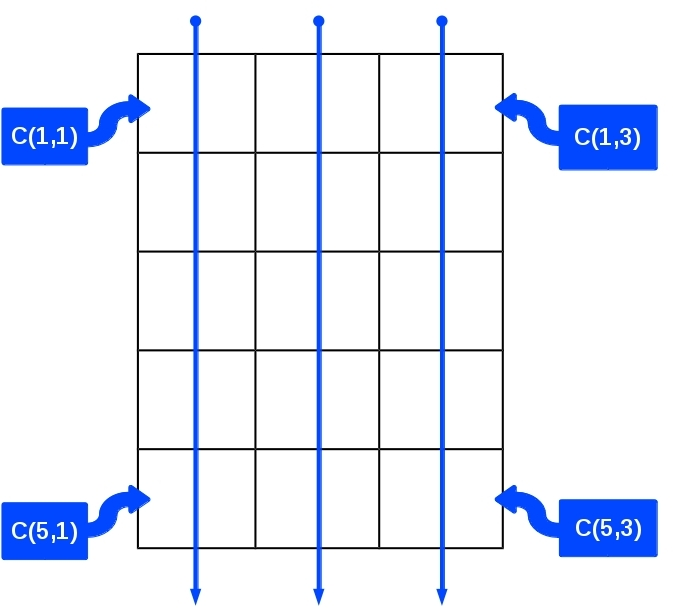
\includegraphics[width=6cm,clip=true]{./graphics/array5}
  \end{center}
\end{frame}

\begin{frame}[fragile,allowframebreaks]{Array Constructors}
  \begin{itemize}
    \item Used to give arrays or sections of arrays specific values
      \begin{lstlisting}[language={[90]Fortran},basicstyle=\fontsize{6}{7}\selectfont\ttfamily]
implicit none
integer :: i
integer, dimension(10) :: ints
character(len=5),dimension(3) :: colors
real, dimension(4) :: height
height = (/5.10, 5.4, 6.3, 4.5 /)
colors = (/'red  ', 'green', 'blue ' /)
ints = (/ 30, (i = 1, 8), 40 /)
      \end{lstlisting}
    \item constructors and array sections must conform.
    \item[] \lstfortran{ints = (/ 30, (i = 1, 10), 40/)} is invalid
    \item strings should be padded so that character variables have correct length.
    \item use \lstfortran{reshape} intrinsic for arrays for higher ranks
    \item \lstfortran{(i = 1, 8)} is an implied \lstfortran{do}.
    \item You can also specify a stride in the implied \lstfortran{do}.
    \item[] \lstfortran{ints = (/ 30, (i = 1, 16, 2), 40 /)}
    \item {\color{red}There should be no space between / and ( or )}
      \framebreak
    \item \lstfortran{reshape(source, shape, pad, order)} constructs an array with a specified shape \lstfortran{shape} starting from the elements in a given array \lstfortran{source}.
    \item If \lstfortran{pad} is not included then the size of \lstfortran{source} has to be at least \lstfortran{product (shape)}. 
    \item If \lstfortran{pad} is included it has to have the same type as \lstfortran{source}. 
    \item If \lstfortran{order} is included, it has to be an \lstfortran{integer} array with the same shape as \lstfortran{shape} and the values must be a permutation of (1,2,3,...,N), where N (max value is 7) is the number of elements in \lstfortran{shape}.
  \end{itemize}
  \begin{columns}[t]
    \column{2cm}
    {\tiny
      \[ \left( \begin{array}{ccc}
        0 & 0 & 0 \\
        0 & a & a \\
        a & 0 & a \\
        a & a & 0
      \end{array}\right) \]
    }
    \column{4cm}
    \begin{lstlisting}[language={[90]Fortran},basicstyle=\fontsize{6}{7}\selectfont\ttfamily]
  rcell = reshape( (/ &
       0.d0, 0.d0, a,    a,   &
       0.d0, a,    0.d0, a,   &
       0.d0, a,    a,    0.d0 &
       /),(/4,3/) )
    \end{lstlisting}
    \column{4cm}
    \begin{lstlisting}[language={[90]Fortran},basicstyle=\fontsize{6}{7}\selectfont\ttfamily]
  rcell = reshape( (/ &
       0.d0, 0.d0, 0.d0 &
       0.d0, a   , a    &
       a,    0.d0, a    &
       a,    a,    0.d0 &
       /),(/4,3/),order=(/2,1/))
    \end{lstlisting}
  \end{columns}
  \begin{itemize}
    \item In Fortran, for a multidimensional array, the first dimension has the fastest index while the last dimension has the slowest index i.e. memory locations are continuous for the last dimension. 
    \item The \lstfortran{order} statement allows the programmer to change this order. The last example above sets the memory location order which is consistent to that in C/C++.
    \item Arrays can be initialized as follows during variable declaration
  \end{itemize}
  \begin{lstlisting}[language={[90]Fortran},basicstyle=\fontsize{6}{7}\selectfont\ttfamily]
 integer, dimension(4) :: imatrix = (/ 2, 4, 6, 8/)
 character(len=*),dimension(3) :: colors = (/'red  ', 'green', 'blue '/)}
 ! All strings must be the same length}
 real, dimension(4) :: height = (/5.10, 5.4, 6.3, 4.5/)
 integer, dimension(10) :: ints = (/ 30, (i = 1, 8), 40/)
 real, dimension(4,3), parameter :: rcell = reshape( (/0.d0, 0.d0, 0.d0, 0.d0,\&
   a, a, a,0.d0, a, a, a, 0.d0 /),(/4,3/),order=(/2,1/)) 
  \end{lstlisting}
\end{frame}

\begin{frame}[fragile]{Array Syntax}
  \begin{itemize}
    \item Arrays can be treated as a single variable when performing operations
    \begin{enumerate}
      \item set whole array to a constant: \lstfortran{a = 0.0}
      \item can use intrinsic operators between conformable arrays (or sections)
      \item[] {\lstfortran{ b = c * d + b**2 }}
      \item[] this is equivalent to
        \begin{lstlisting}[language={[90]Fortran},mathescape]
b(-4,0) = c(1,1) * d(4,2) + b(-4,0)**2 
b(-3,0) = c(2,1) * d(5,2) + b(-3,0)**2 
$\cdots$
b(-4,0) = c(1,1) * d(4,2) + b(-4,0)**2 
b(-4,1) = c(1,2) * d(4,3) + b(-4,1)**2 
$\cdots$
b(-3,2) = c(4,3) * d(7,4) + b(-3,2)**2 
b(-4,2) = c(5,3) * d(8,4) + b(-4,2)**2 
        \end{lstlisting}
      \item elemental intrinsic functions can be used: \lstfortran{ b = sin(c) + cos(d)}
      \item All operations/functions are applied element by element
    \end{enumerate}
  \end{itemize}
\end{frame}

\begin{frame}[fragile,allowframebreaks]
  \frametitle{\small Array Sections}
  \begin{columns}[t]
    \column{7cm}
    \begin{itemize}
      \scriptsize
      \item[] \lstfortran{real, dimension(6:6) :: a}
      \item {\lstfortran{a(1:3,1:3) = a(1:6:2,2:6:2)}} and
      \item[] {\lstfortran{a(1:3,1:3) = 1.0 }} are valid
      \item {\lstfortran{a(2:5,5) = a(2:5,1:6:2)}} and
      \item[] {\lstfortran{a(2:5,1:6:2) = a(1:6:2,2:6:2)}} are not
      \item {\lstfortran{a(2:5,5)}} is a 1D section while 
      \item[] {\lstfortran{a(2:5,1:6:2)}} is a 2D section
    \end{itemize}
    \column{4cm}
    \begin{center}
      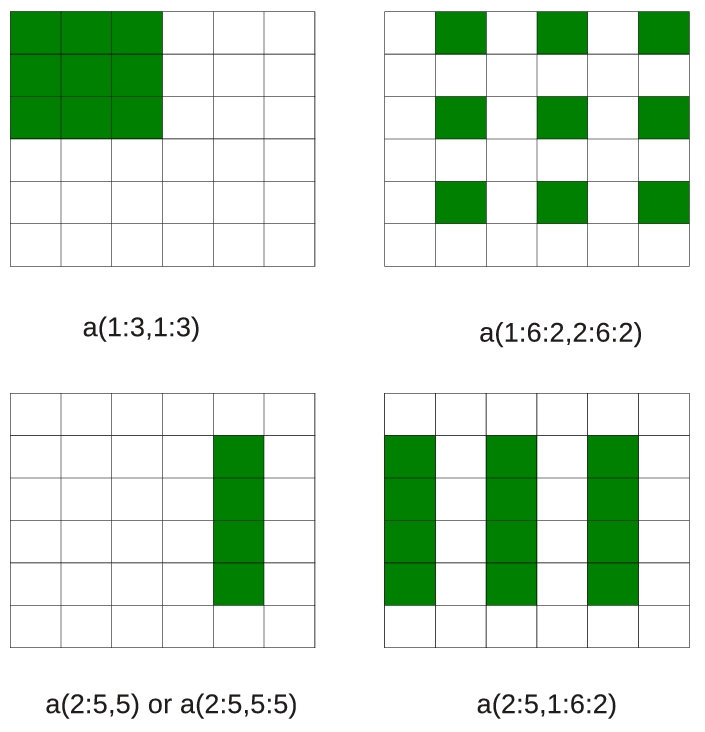
\includegraphics[width=4cm,clip=true]{./graphics/array6}
    \end{center}
  \end{columns}
  \begin{itemize}
    \scriptsize
    \item The general form for specifying sub-arrays or sections is
    \item[] \textit{[<bound1>]:[<bound2>][:<stride>]}
    \item The section starts at \textit{<bound1>} and ends at or before \textit{<bound2>}.
    \item \textit{<stride>} is the increment by which the locations are selected, by default \textit{stride=1}
    \item \textit{<bound1>}, \textit{<bound2>}, \textit{<stride>} must all be scalar integer expressions.
  \end{itemize}

  \begin{lstlisting}[language={[90]Fortran}]
real, dimension(1:20) :: a
integer :: m,n,k
  \end{lstlisting}
  \begin{center}
    \scriptsize
    \begin{tabular}{lcl}
      {\lstfortran{a(:)}} &  & the whole array \\
      {\lstfortran{a(3:9)}} &  & elements 3 to 9 in increments of 1 \\
      {\lstfortran{a(3:9:1)}} &  & as above \\
      {\lstfortran{a(m:n)}} &  & elements m through n\\
      {\lstfortran{a(m:n:k)}} &  & elements m through n in increments of k \\
      {\lstfortran{a(15:3:-2)}} &  & elements 15 through 3 in increments of -2 \\
      {\lstfortran{a(15:3)}} &  & zero size array \\
      {\lstfortran{a(m:)}} &  & elements m through 20, default upper bound \\
      {\lstfortran{a(:n)}} &  & elements 1, default lower bound through n \\
      {\lstfortran{a(::2)}} &  & all elements from lower to upper bound in increments of 2 \\
      {\lstfortran{a(m:m)}} &  & 1 element section \\
      {\lstfortran{a(m)}} &  & array element not a section \\
      are valid sections. & & \\
    \end{tabular}
  \end{center}
\end{frame}

\begin{frame}[fragile,allowframebreaks]
  \frametitle{\small Array I/O}
  \begin{itemize}
    \item[] \lstfortran{real,dimension(4,4) :: a}
    \item Arrays are printed in the order that they appear in memory
    \item[] \lstfortran{print *, a}
    \item[] would produce on output
    \item[] \lstinline[mathescape]{a(1,1),a(2,1),a(3,1),a(4,1),a(1,2),a(2,2),$\cdots$,a(3,4),a(4,4)}
    \item[] \lstfortran{read *, a}
    \item[] would read from input and assign array elements in the same order as above
    \item The order of array I/O can be changed using intrinsic functions such as \lstfortran{reshape, transpose} or \lstfortran{cshift}.
      \framebreak
    \item Example: consider a 3x3 matrix
      \begin{center}
        \begin{tabular}{|c|c|c|}
          \hline
          1 & 4 & 7 \\ \hline
          2 & 5 & 8 \\ \hline
          3 & 6 & 9 \\ \hline
        \end{tabular}
      \end{center}
      \item The following print statements
        \begin{lstlisting}[language={[90]Fortran}]
 print *, 'array element   = ',a(3,3)
 print *, 'array section   = ',a(:,2)
 print *, 'sub-array       = ',a(:3,:2)
 print *, 'whole array     = ',a
 print *, 'array transpose = ',transpose(a)
        \end{lstlisting}
      \item would produce the following output
        \begin{Verbatim}[formatcom=\color{indigo}]
 array element   = 9
 array section   = 4 5 6
 sub-array       = 1 2 3 4 5 6
 whole array     = 1 2 3 4 5 6 7 8 9
 array transpose = 1 4 7 2 5 8 3 6 9
        \end{Verbatim}
    \end{itemize}
\end{frame}

\begin{frame}[allowframebreaks]{Array Intrinsic Functions}
  \begin{description}
    \item[{size(x[,n])}] The size of x (along the $n^{th}$ dimension, optional)
    \item[shape(x)] The shape of x
    \item[{lbound(x[,n])}] The lower bound of x
    \item[{ubound(x[,n])}] The upper bound of x
    \item[minval(x)] The minimum of all values of x
    \item[maxval(x)] The maximum of all values of x
    \item[minloc(x)] The indices of the minimum value of x
    \item[maxloc(x)] The indices of the maximum value of x
    \item[{sum(x[,n])}] The sum of all elements of x (along the $n^{th}$ dimension, optional)
    \item[] $sum(x) = \sum_{i,j,k,\cdots}x_{i,j,k,\cdots}$
      \framebreak
    \item[{product(x[,n])}] The product of all elements of x (along the $n^{th}$ dimension, optional)
    \item[] $prod(x) = \prod_{i,j,k,\cdots}x_{i,j,k,\cdots}$
    \item[transpose(x)] Transpose of array x: $ x_{i,j}\Rightarrow x_{j,i}$
    \item[dot\_product(x,y)] Dot Product of arrays x and y: $ \sum_{i} x_i* y_i $
    \item[matmul(x,y)] Matrix Multiplication of arrays x and y which can be 1 or 2 dimensional arrays: $ z_{i,j} = \sum_k x_{i,k} * y_{k,j}$
    \item[conjg(x)] Returns the conjugate of x: $ a + \imath b \Rightarrow a - \imath b$
    \item[cshift(ARRAY, SHIFT, dim)] perform a circular shift by SHIFT positions to the left on array ARRAY along the dim$^{\mathrm{th}}$ dimension
  \end{description}
\end{frame}

\begin{frame}[fragile,allowframebreaks]{Allocatable Arrays}
  \begin{block}{\scriptsize Why?}
    \begin{itemize}
      \item At compile time we may not know the size an array needs to be
      \item We may want to change the problem size without recompiling
      \item The molecular dynamics code was written for 4000 atoms. If you want to run a simulation for 256 and 1024 atoms, do you need to recompile and create two executables?
    \end{itemize}
  \end{block}
  \begin{itemize}
    \item Allocatable arrays allow us to set the size at run time.
    \item[] \lstfortran{real, allocatable :: force(:,:)}
    \item[] \lstfortran{real, dimension(:), allocatable :: vel}
    \item We set the size of the array using the allocate statement.
    \item[] \lstfortran{allocate(force(natoms,3))}
    \item We may want to change the lower bound for an array
    \item[] \lstfortran{allocate(grid(-100,100))}
    \item We may want to use an array once somewhere in the program, say during initialization. Using allocatable arrays also us to dynamically create the array when needed and when not in use, free up memory using the \lstfortran{deallocate} statement
    \item[] \lstfortran{deallocate(force,grid)}
    \item Sometimes, we want to check whether an array is allocated or not at a particular part of the code
    \item Fortran provides an intrinsic function, \lstfortran{allocated} which returns a scalar logical value reporting the status of an array
    \item[] \lstfortran{if ( allocated(grid) ) deallocate(grid)}
    \item[] \lstfortran{if ( .not. allocated(force) ) allocate(force(natoms,3))}
  \end{itemize}
\end{frame}

\begin{frame}[fragile]{Masked Array Assignment: Where Statement}
  \begin{itemize}
    \item Masked array assignment is achieved using the \lstfortran{where} statement
    \item[] \lstfortran{where ( c < 2 ) a = b/c }
    \item[] the left hand side of the assignment must be array valued.
    \item[] the mask (logical expression) and the right hand side of the assignment must all conform
    \item Fortran 95/2003 introduced the \lstfortran{where ... elsewhere ... end where} functionality
    \item \lstfortran{where} statement cannot be nested
  \end{itemize}
  \begin{columns}[t]
    \column{4.8cm}
    \begin{lstlisting}[language={[90]Fortran},basicstyle=\fontsize{6}{7}\selectfont\ttfamily]
 ! Apply PBC to coordinates
 where ( coord(i,:) > boxl(:) )
    coord(i,:) = coord(i,:) - boxl(:)
 elsewhere ( coord(i,:) < 0d0 )
    coord(i,:) = coord(i,:) + boxl(:)
 end where
    \end{lstlisting}
    \column{5.5cm}
    \begin{lstlisting}[language={[90]Fortran},basicstyle=\fontsize{6}{7}\selectfont\ttfamily]
 ! Apply PBC to coordinates
 do j = 1, 3
    if ( coord(i,j) > boxl(j) ) then
       coord(i,j) = coord(i,j) - boxl(j)
    else if ( coord(i,j) < 0d0 ) then
       coord(i,j) = coord(i,j) + boxl(j)
    endif
 end do
    \end{lstlisting}
  \end{columns}
\end{frame}

%\begin{frame}[fragile]{Vector valued subscripts}
%  \begin{itemize}
%    \item A 1D array can be used to subscript an array in a dimension
%    \item[] \lstfortran{real, dimension(15) :: a}
%    \item[] \lstfortran{integer, dimension(5) :: v = (/ 1,4,8,10,15/)}
%    \item[] \lstfortran{integer, dimension(3) :: w = (/ 1,2,3/)}
%    \item[$\vardiamond$] {\lstfortran{a(v)}} is {\lstfortran{a(1), a(4), a(8), a(10)}} and {\lstfortran{a(15)}}
%    \item[$\vardiamond$] {\lstfortran{a(v) = 1.2}} is valid
%    \item[$\vardiamond$] only 1D vector subscripts are allowed
%    \item[] {\lstfortran{a(1) = prod(c(v,w))}}
%  \end{itemize}
%\end{frame}

\section{Procedures}
\begin{frame}[fragile,allowframebreaks]{Program Units}

  \begin{itemize}
    \item Most programs are hundreds or more lines of code.
    \item Use similar code in several places.
    \item A single large program is extremely difficult to debug and maintain.
    \item Solution is to break up code blocks into procedures
    \begin{description}
      \item[Subroutines:] Some out-of-line code that is called exactly where it is coded
      \item[Functions:] Purpose is to return a result and is called only when the result is needed
      \item[Modules:] A module is a program unit that is not executed directly, but contains data specifications
and procedures that may be utilized by other program units via the use statement.
    \end{description}
  \end{itemize}

  \framebreak

  \begin{lstlisting}[language={[90]Fortran},basicstyle=\fontsize{5}{6}\selectfont\ttfamily,mathescape]
program main 

  use module1 ! specify which modules to use

  implicit none  ! implicit typing is not recommended
  variable declarations  ! declare all variables used in the program

  $\vdots$  ! executable statements in seqeunce

  call routine1(arg1,arg2,arg3) ! call subroutine routine1 with arguments
  $\vdots$
  abc = func(arg1,arg2) ! abc is some function of arg1 and arg2
  $\vdots$

  contains  ! internal procedures are listed below

    subroutine routine1(arg1,arg2)  ! subroutine routine1 contents go here
      $\vdots$
    end subroutine routine1  ! all program units must have an end statement

    function func(arg1,arg2) ! function func1 contents go here
      ...
    end function func

  end program main
  \end{lstlisting}
  \framebreak
  \lstinputlisting[language={[90]Fortran},basicstyle=\fontsize{4}{5}\selectfont\ttfamily]{./Exercise/MolDyn/orig/md-orig.f90}
\end{frame}

\begin{frame}[fragile, allowframebreaks]{Subroutines}
  \begin{itemize}
    \item Call Statement: 
      \begin{itemize}
        \item The \lstfortran{call} statement evaluates its arguments and transfers control to the subroutine\\
        \item Upon return, the next statement is executed.
      \end{itemize}
    \item SUBROUTINE Statement:
      \begin{itemize}
        \item The \lstfortran{subroutine} statement declares the procedure and its arguments.\\
        \item These are also known as dummy arguments.
      \end{itemize}
    \item The subroutine's interface is defined by
      \begin{itemize}
        \item The \lstfortran{subroutine} statement itself
        \item The declarations of its dummy arguments
        \item Anything else that the subroutine uses
%        \item In the previous example, the \lstfortran{subroutine verlet} is an external procedure and can be called by any program unit with the program.
      \end{itemize}
      \framebreak
    \item Statement Order
      \begin{enumerate}
        \item A \lstfortran{subroutine} statement starts a subroutine
        \item Any \lstfortran{use} statements come next
        \item \lstfortran{implicit none} comes next, followed by
        \item rest of the declarations,
        \item executable statements
        \item End with a \lstfortran{end subroutine} statement
      \end{enumerate}
    \item Dummy Arguments
      \begin{itemize}
        \item Their names exist only in the procedure and are declared as local variables.
        \item The dummy arguments are associated with the actual arguments passed to the subroutines.
        \item The dummy and actual argument lists must match, i.e. the number of arguments must be the same and each argument must match in type and rank.
      \end{itemize}
  \end{itemize}
  \framebreak
  \vspace{-0.5cm}
  \begin{columns}[t]
    \column{0.5\textwidth}
      \lstinputlisting[language={[90]Fortran},basicstyle=\fontsize{3.5}{4}\selectfont\ttfamily]{./Exercise/MolDyn/code/verlet.f90}
    \column{0.5\textwidth}
      \begin{lstlisting}[language={[90]Fortran},basicstyle=\fontsize{3.5}{4.5}\selectfont\ttfamily,mathescape]
program md

$\cdots$

  real(dp), dimension(:,:), allocatable :: coord_t0, coord
  real(dp), dimension(:,:), allocatable :: vel_t0, vel
  real(dp), dimension(:,:), allocatable :: acc_t0, acc, force
  real(dp) :: pener

  interface
     $\cdots$
     subroutine verlet(coord, coord_t0, vel_t0, vel, acc_t0, acc, force, pener)
       use precision
       implicit none
       real(dp), dimension(:,:), intent(in) :: coord_t0, vel_t0, acc_t0
       real(dp), dimension(:,:), intent(out) :: coord, vel, acc, force
       real(dp), intent(out) :: pener
     end subroutine verlet
     $\cdots$
  end interface

  $\cdots$

  do istep = 1, nstep

     ! Set coordinates, velocity, acceleration and force at next time step to zero
     coord = 0d0 ; vel = 0d0 ; acc = 0d0
     force = 0d0 ; pener = 0d0
     
     ! Get new atom positions from Velocity Verlet Algorithm
     call verlet(coord, coord_t0, vel_t0, vel, acc_t0, acc, force, pener)

     $\cdots$
  end do

  ! Free up memory
  deallocate(coord_t0,vel_t0,acc_t0,coord,vel,acc,force)

end program md

      \end{lstlisting}
  \end{columns}
\end{frame}

\begin{frame}[fragile]{Internal Procedures}
  \begin{itemize}
    \item Internal procedures appear just before the last \lstfortran{end} statement and are preceeded by the \lstfortran{contains} statement.
    \item Internal procedures can be either subroutines or functions which can be accessed only by the program, subroutine or module in which it is present
    \item Internal procedures have declaration of variables passed on from the parent program unit
    \item If an internal procedure declares a variable which has the same name as a variable from the parent program unit then this supersedes the variable from the outer scope for the length of the procedure.
%    \item i.e. internal procedures are not global and connot be called by other program units.
  \end{itemize}
\end{frame}

\begin{frame}[fragile]{Functions}
  \begin{itemize}
    \item \lstfortran{function}s operate on the same principle as \lstfortran{subroutine}s
    \item The only difference is that \lstfortran{function} returns a value and does not involve the \lstfortran{call} statement 
  \end{itemize}
  \lstinputlisting[language={[90]Fortran},basicstyle=\fontsize{3.5}{4.5}\selectfont\ttfamily,multicols=2]{./Exercise/MolDyn/code/potential.f90}
\end{frame}

\begin{frame}[fragile]{Array-valued Functions}
  \begin{itemize}
    \item \lstfortran{function} can also return arrays
  \end{itemize}
%  \begin{columns}[t]
%    \column{5.5cm}
%    \begin{eblock}{Example}
      \begin{lstlisting}[language={[90]Fortran},basicstyle=\fontsize{4}{5}\selectfont\ttfamily,multicols=2]
module potential
  use precision
  implicit none
  real(dp) :: r2, r6, d2, d
  real(dp), parameter :: de = 0.176d0, a = 1.4d0, re = 1d0
  real(dp) :: exparre
  
contains
  subroutine lennard_jones(r,f,p)
    ! Lennard Jones Potential
    ! V = 4 * epsilon * [ (sigma/r)**12 - (sigma/r)**6 ]
    !   = 4 * epsilon * (sigma/r)**6 * [ (sigma/r)**2 - 1 ]
    !   = 4 * r**(-6) * [ r**(-2) - 1 ] for epsilon=sigma=1
    ! F_i = 48 * epsilon * (sigma/r)**6 * (1/r**2) * [ ( sigma/r)** 6 - 0.5 ] * i where i = x,y,z
    !     = 48 * r**(-8) * [ r**(-6) - 0.5 ] * i  for epsilon=sigma=1    implicit none
    implicit none
    real(dp), dimension(:), intent(in) :: r
    real(dp), dimension(:), intent(out) :: f
    real(dp), intent(out) :: p

    r2 = 1.d0 / dot_product(r,r)
    r6 = r2 ** 3

    f = dvdr_lj(r2, r6, r)
    p = pot_lj(r2, r6)
  end subroutine lennard_jones

  subroutine morse(r,f,p)
    ! Morse Potential
    ! V = D * [ 1 - exp(-a*(r - re)) ]^2
    ! F_i = 2*D * [ 1 - exp(-a*(r - re)) ] * a exp(-a*(r-re)) * i / r  
    implicit none
    real(dp), dimension(:), intent(in) :: r
    real(dp), dimension(:), intent(out) :: f
    real(dp), intent(out) :: p

    d2 = dot_product(r,r)
    d = sqrt(d2)
    exparre = exp( -a * (d - re ))
    
    f = dvdr_mp(exparre,r)
    p = pot_mp(exparre)
  end subroutine morse

  function pot_lj(r2, r6)
    implicit none
    real(dp), intent(in) :: r2, r6
    real(dp) :: pot_lj
    pot_lj = 4d0 * r6 * ( r6 - 1.d0 )
  end function pot_lj
  function pot_mp(exparre)
    implicit none
    real(dp), intent(in) :: exparre
    real(dp) :: pot_mp
    pot_mp = de * ( 1d0 - exparre )**2
  end function pot_mp

  function dvdr_lj(r2,r6,r)
    implicit none
    real(dp), intent(in) :: r2, r6, r
    real(dp), dimension(size(r)) :: dvdr_lj
    dvdr_lj = 48d0 * r2 * r6 * ( r6 - 0.5d0 ) * r
  end function dvdr_lj
  function dvdr_mp(exparre,r)
    implicit none
    real(dp), intent(in) :: exparre, r
    real(dp), dimension(size(r)) :: dvdr_mp
    dvdr_mp = 2d0 * de * a * (1d0 - exparre) * exparre * r
  end function dvdr_mp
end module potential
      \end{lstlisting}
%    \end{eblock}
%    \column{5.5cm}
%  \end{columns}
\end{frame}

\begin{frame}[fragile]{Recursive Procedures}
  \begin{itemize}
    \item In Fortran 90, recursion is supported as a feature
    \begin{enumerate}
      \item \lstfortran{recursive} procedures call themselves
      \item \lstfortran{recursive} procedures must be declared explicitly
      \item \lstfortran{recursive function} declarations must contain a \lstfortran{result} keyword, and 
      \item one type of declaration refers to both the function name and the result variable.
    \end{enumerate}
  \end{itemize}    
  \begin{columns}[t]
    \column{6cm}
      \lstinputlisting[language={[90]Fortran},basicstyle=\fontsize{4.5}{5}\selectfont\ttfamily]{./Exercise/factorial.f90}
    \column{5cm}
      \begin{Verbatim}[fontsize=\fontsize{4.5}{5}\selectfont,formatcom=\color{indigo}]
[apacheco@qb4 Exercise] ./factorial
 enter integer whose factorial you want to calculate
10 
   10! =              3628800
[apacheco@qb4 Exercise] ./fact1
 Enter an integer < 15
10
  10!=        3628800
        \end{Verbatim}
    \end{columns}
\end{frame}

\begin{frame}[fragile]{Argument Association}
  \begin{itemize}
    \item Recall from MD code example the invocation
    \item[] \lstfortran{call linearmom(vel_t0)}
    \item and the subroutine declaration
    \item[] \lstfortran{subroutine linearmom(vel)}
    \item[]
    \item {\lstfortran{vel_t0}} is an actual argument and is associated with the dummy argument {\lstfortran{vel}}
    \item In {\lstfortran{subroutine linearmom}}, the name {\lstfortran{vel}} is an alias for {\lstfortran{vel_t0}}
    \item If the value of a dummy argument changes, then so does the value of the actual argument
    \item {\color{red}The actual and dummy arguments must correspond in type, kind and rank.}
  \end{itemize}
\end{frame}

\begin{frame}[fragile]
  \frametitle{\small Local Objects}
  \begin{columns}
    \column{6cm}
    \begin{itemize}
      \item In \lstfortran{subroutine linearmom},
      \item[] \lstfortran{i} and \lstfortran{vcm} are local objects.
      \item Local Objects 
      \begin{enumerate}
        \item[$\vardiamond$] are created each time a procedure is invoked
        \item[$\vardiamond$] are destroyed when the procedure completes
        \item[$\vardiamond$] do not retain their values between calls
        \item[$\vardiamond$] do not exist in the programs memory between calls.
      \end{enumerate}
    \end{itemize}
    \column{4.5cm}
    \begin{eblock}{Example}
      \lstinputlisting[language={[90]Fortran},basicstyle=\fontsize{4}{5}\selectfont\ttfamily]{./Exercise/MolDyn/code/linearmom.f90}
    \end{eblock}
  \end{columns}
\end{frame}

\begin{frame}[fragile,allowframebreaks]{Optional \& Keyword Arguments}
  \begin{itemize}
    \item Optional Arguments
      \begin{itemize}
        \item allow defaults to be used for missing arguments
        \item make some procedures easier to use
      \end{itemize}
    \item once an argument has been omitted all subsequent arguments must be keyword arguments
    \item the \lstfortran{present} intrinsic can be used to check for missing arguments
    \item if used with external procedures then the \lstfortran{interface} must be explicit within the procedure in which it is invoked.
      \begin{columns}[t]
        \column{0.5\textwidth}
        \begin{lstlisting}[language={[90]Fortran},basicstyle=\fontsize{4}{5}\selectfont\ttfamily,mathescape]
subroutine get_temp(vel,boltz)
  use precision
  use param, only : natom, avtemp, mass, kb
  implicit none
  real(dp), dimension(:,:), intent(in) :: vel
  real(dp), optional :: boltz
  integer(ip) :: i
  real(dp) :: ke

  if (present(boltz))kb = boltz
  ke = 0d0
  do i = 1, natom
     ke = ke + dot_product(vel(i,:),vel(i,:))
  end do
  avtemp = mass * ke / ( 3d0 * kb * real( natom - 1, dp))
  
end subroutine get_temp


        \end{lstlisting}
%        \lstinputlisting[language={[90]Fortran},basicstyle=\fontsize{4}{5}\selectfont\ttfamily]{./Exercise/MolDyn/ccode/get_temp.f90}
        \column{0.5\textwidth}
        \begin{lstlisting}[language={[90]Fortran},basicstyle=\fontsize{4}{5}\selectfont\ttfamily,mathescape]
subroutine initialize(coord_t0, vel_t0, acc_t0)
$\cdots$
  interface
     subroutine linearmom(vel)
       use precision
       implicit none
       real(dp), dimension(:,:), intent(inout) :: vel
     end subroutine linearmom
     subroutine get_temp(vel, boltz)
       use precision
       implicit none
       real(dp), dimension(:,:), intent(in) :: vel
       real(dp), optional :: boltz
     end subroutine get_temp
  end interface
$\cdots$
  call get_temp(vel_t0)
$\cdots$
        \end{lstlisting}
      \end{columns}
    \item Keyword Arguments
      \begin{itemize}
        \item allow arguments to be specified in any order
        \item makes it easy to add an extra argument - no need to modify any calls
        \item helps improve readability of the program
        \item are used when a procedure has optional arguments
      \end{itemize}
    \item once a keyword is used, all subsequent arguments must be keyword arguments
    \item if used with external procedures then the \lstfortran{interface} must be explicit within the procedure in which it is invoked.
  \end{itemize}

  \begin{columns}
    \column{5.5cm}
    \begin{lstlisting}[language={[90]Fortran},basicstyle=\fontsize{5}{6}\selectfont\ttfamily]
subroutine initialize(coord, vel, acc)

  ...
  real(dp),dimension(:,:), intent(out) :: coord, vel, acc
  ...
end subroutine initialize
    \end{lstlisting}
    \column{5.5cm}
    \begin{lstlisting}[language={[90]Fortran},basicstyle=\fontsize{5}{6}\selectfont\ttfamily]
program md
         ...
     call initialize(coord_t0, vel_t0, acc_t0)
         ...
end program md
    \end{lstlisting}
  \end{columns}
  \framebreak
  \begin{itemize}
    \item \lstfortran{subroutine initialize} can be invoked using 
    \begin{enumerate}
      \item using the positional argument invocation
      \item using keyword arguments
    \end{enumerate}
    \begin{lstlisting}[language={[90]Fortran},basicstyle=\fontsize{7}{8}\selectfont\ttfamily,mathescape]
program md
$\cdots$
  interface
     subroutine initialize(coord, vel, acc)
       use precision
       implicit none
       real(dp), dimension(:,:), intent(out) :: coord, vel, acc
     end subroutine initialize
  end interface
$\cdots$
! All three calls give the same result.
  call initialize(coord_t0, vel_t0, acc_t0)
  call initialize(coord=coord_t0, acc=acc_t0, vel=vel_t0)
  call initialize(coord_t0, acc=acc_t0, vel=vel_t0)
$\cdots$
    \end{lstlisting}
  \end{itemize}
\end{frame}

\begin{frame}[fragile]{Dummy Array Arguments}
  \begin{itemize}
    \item There are two main types of dummy array argument:
    \begin{enumerate}
      \item \textit{explicit-shape}: all bounds specified
%      \item[] \lstfortran{real, dimension(4,4), intent(in) :: explicit_shape}
      \item[] \lstinline[language={[90]Fortran},basicstyle=\fontsize{7}{8}\selectfont\ttfamily]{real, dimension(4,4), intent(in) :: explicit_shape}
      \item[] The actual argument that becomes associated with an explicit shape dummy must conform in size and shape
      \item \textit{assumed-shape}: no bounds specified, all inherited from the actual argument
      \item[] \lstinline[language={[90]Fortran},basicstyle=\fontsize{7}{8}\selectfont\ttfamily]{real, dimension(:,:), intent(out) :: assumed_shape}
      \item[] An explicit interface must be provided
      \item \textit{assumed-size}: final dimension is specified by $\ast$
      \item[] \lstinline[language={[90]Fortran},basicstyle=\fontsize{7}{8}\selectfont\ttfamily]{real :: assumed_size(dim1,dim2,*)}
      \item[] Commomly used in FORTRAN, use assumed-shape arrays in Modern Fortran.
    \end{enumerate}
    \item dummy arguments cannot be (unallocated) allocatable arrays.
  \end{itemize}
\end{frame}

\begin{frame}[fragile]{Explicit-shape Arrays}
  \begin{lstlisting}[language={[90]Fortran},basicstyle=\fontsize{4.5}{5.5}\selectfont\ttfamily,mathescape]
program md
  use precision
  use param
  implicit none
  integer(ip) :: n, i, j, k, l
  real(dp), dimension(:,:), allocatable :: coord_t0, vel_t0, acc_t0
  real(dp), dimension(:,:), allocatable :: coord, vel, acc, force
  $\cdots$
  ! Allocate arrays
  allocate(coord(natom,3), coord_t0(natom,3))
  allocate(vel(natom,3), vel_t0(natom,3))
  allocate(acc(natom,3), acc_t0(natom,3))
  allocate(force(natom,3))

  !=================================================
  ! Initialize coordinates and random velocities
  !=================================================

  call initialize(coord_t0, vel_t0, acc_t0)

  $\cdots$
end program md

subroutine initialize(coord_t0, vel_t0, acc_t0)
  use precision
  use param, only : natom, npartdim, alat, rcell
  implicit none
  real(dp), dimension(natom,3) :: coord_t0, vel_t0, acc_t0
  integer(ip) :: n, i, j, k, l

  ! Set initial coordinates, velocity and acceleration to zero
  coord_t0 = 0d0 ; vel_t0 = 0d0 ; acc_t0 = 0d0
  $\cdots$
end subroutine initialize
  \end{lstlisting}
\end{frame}

\begin{frame}[fragile]{Assumed-Shape Arrays}
  \begin{lstlisting}[language={[90]Fortran},basicstyle=\fontsize{4}{5}\selectfont\ttfamily,mathescape]
program md
  use precision
  use param
  implicit none
  integer(ip) :: n, i, j, k, l
  real(dp), dimension(:,:), allocatable :: coord_t0, vel_t0, acc_t0
  real(dp), dimension(:,:), allocatable :: coord, vel, acc, force
  $\cdots$
  interface
     subroutine initialize(coord_t0, vel_t0, acc_t0)
       use precision
       implicit none
       real(dp), dimension(:,:), intent(out) :: coord_t0, vel_t0, acc_t0
     end subroutine initialize
     $\cdots$
  end interface
  $\cdots$
  ! Allocate arrays
  allocate(coord(natom,3), coord_t0(natom,3))
  allocate(vel(natom,3), vel_t0(natom,3))
  allocate(acc(natom,3), acc_t0(natom,3))
  allocate(force(natom,3))

  !=================================================
  ! Initialize coordinates and random velocities
  !=================================================

  call initialize(coord_t0, vel_t0, acc_t0)
  $\cdots$
end program md

subroutine initialize(coord_t0, vel_t0, acc_t0)
  use precision
  use param, only : natom, npartdim, alat, rcell
  implicit none
  real(dp), dimension(:,:), intent(out) :: coord_t0, vel_t0, acc_t0
  integer(ip) :: n, i, j, k, l

  ! Set initial coordinates, velocity and acceleration to zero
  coord_t0 = 0d0 ; vel_t0 = 0d0 ; acc_t0 = 0d0
  $\cdots$
end subroutine initialize
  \end{lstlisting}
%  \begin{itemize}
%    \scriptsize
%    \item The actual arguments cannot be vector subscribed array.
%    \item The actual argument cannot be an assumed-size array
%    \item In the procedure, bounds begin at 1
%    \item If using external procedure, an explicit interface must be described
%  \end{itemize}
\end{frame}

\begin{frame}[fragile]{Automatic Arrays}
  \begin{itemize}
    \item Automatic Arrays: Arrays which depend on dummy arguments
    \begin{enumerate}
      \scriptsize
      \item their size is determined by dummy arguments
      \item they cannot have the \lstfortran{save} attribute or be initialized.
    \end{enumerate}
    \item The \lstfortran{size} intrinsic or dummy arguments can be used to declare automatic arrays.
      \begin{lstlisting}[language={[90]Fortran},mathescape,basicstyle=\fontsize{6}{7}\selectfont\ttfamily]
program main
  implicit none
  integer :: i,j
  real, dimension(5,6) :: a
  $\vdots$
  call routine(a,i,j)
  $\vdots$
  contains
    subroutine routine(c,m,n)
      integer :: m,n
      real, dimension(:,:), intent(inout) :: c   ! assumed shape array
      real :: b1(m,n)                            ! automatic array
      real, dimension(size(c,1),size(c,2)) :: b2 ! automatic array
      $\vdots$
    end subroutine routine
end program main
      \end{lstlisting}
  \end{itemize}
\end{frame}

\begin{frame}[fragile]{Save Attribute and Arrays}
  \begin{itemize}
    \item Declaring a variable (or array) as \lstfortran{save} gives it a static storage memory.
    \item i.e information about variables is retained in memory between procedure calls.
      \begin{lstlisting}[language={[90]Fortran},mathescape,basicstyle=\fontsize{6}{7}\selectfont\ttfamily]
subroutine something(iarg1)
  implicit none
  integer, intent(in) :: iarg1 
  real,dimension(:,:),allocatable,save :: a 
  real, dimension(:,:),allocatable :: b 
  $\vdots$ 
  if (.not.allocated(a))allocate(a(i,j)) 
  allocate(b(j,i))
  $\vdots$
  deallocate(b)
end subroutine something
      \end{lstlisting}
    \item Array {\lstfortran{a}} is saved when {\lstfortran{something}} exits.
    \item Array {\lstfortran{b}} is not saved and needs to be allocated every time in {\lstfortran{something}}  and deallocated, to free up memory, before {\lstfortran{something}} exits.
  \end{itemize}
\end{frame}

\begin{frame}[fragile]{Intent}
  \begin{itemize}
    \item \lstfortran{intent} attribute was introduced in Fortran 90 and is recommended as it
    \begin{enumerate}
      \item allows compilers to check for coding errors
      \item facilitates efficient compilation and optimization
    \end{enumerate}
    \item Declare if a parameter is
    \begin{enumerate}
      \item[$\vardiamond$]Input: \lstfortran{intent(in)} 
      \item[$\vardiamond$]Output: \lstfortran{intent(out)}
      \item[$\vardiamond$]Both: \lstfortran{intent(inout)}
    \end{enumerate}
    \begin{lstlisting}[language={[90]Fortran},mathescape,basicstyle=\fontsize{6}{7}\selectfont\ttfamily]
subroutine verlet(coord, coord_t0, vel_t0, vel, acc_t0, acc, force, pener)
  use precision
  use param, only : natom, mass, boxl, dt
  implicit none
  real(dp),dimension(:,:), intent(in) :: coord_t0, vel_t0, acc_t0
  real(dp),dimension(:,:), intent(out) :: coord, vel, acc, force
  real(dp), intent(out) :: pener
$\vdots$
end subroutine verlet
    \end{lstlisting}
    \item A variable declared as \lstfortran{intent(in)} in a procedure cannot be changed during the execution of the procedure (see point 1 above)
  \end{itemize}
\end{frame}

\begin{frame}[fragile,allowframebreaks]
  \frametitle{\small Interfaces}
  \begin{itemize}
    \item The \lstfortran{interface} statement is the first statement in an interface block.
    \item The \lstfortran{interface} block is a powerful structure that was introduced in FORTRAN 90.
    \item When used, it gives a calling procedure the full knowledge of the types and characteristics of the dummy arguments that are used inside of the procedure that it references.
    \item This can be a very good thing as it provides a way to execute some safety checks when compiling the program. 
    \item Because the main program knows what argument types should be sent to the referenced procedure, it can check to see whether or not this is the case.
    \item If not, the compiler will return an error message when you attempt to compile the program.
  \end{itemize}
  \framebreak
  \lstinputlisting[language={[90]Fortran},basicstyle=\fontsize{4}{5}\selectfont\ttfamily,multicols=2]{./Exercise/MolDyn/code/verlet1.f90}
  \framebreak
  \vspace{-0.5cm}
  \lstinputlisting[language={[90]Fortran},basicstyle=\fontsize{4}{5}\selectfont\ttfamily,multicols=2]{./Exercise/MolDyn/code/verlet2.f90}
  \vspace{-0.5cm}
  \begin{itemize}
    \scriptsize
    \item Here since \lstfortran{subroutine get_pot\_force} is an internal procedure, no \lstfortran{interface} is required since it is already implicit and all variable declarations are carried over from \lstfortran{subroutine verlet}
  \end{itemize}
\end{frame}

\begin{frame}[fragile,allowframebreaks]{Modules}
  \begin{itemize}
%    \item A module is a program unit that is not executed directly, but contains data specifications and procedures that may be utilized by other program units via the use statement.
    \item Modules were introduced in Fortran 90 and have a wide range of applications.
    \item Modules allow the user to write object based code.
    \item A \lstfortran{module} is a program unit whose functionality can be exploited by other programs which attaches to it via the \lstfortran{use} statement.
    \item A \lstfortran{module} can contain the following
    \begin{enumerate}
      \item global object declaration: replaces Fortran 77 \lstfortran{COMMON} and \lstfortran{INCLUDE} statements
      \item interface declaration: all external procedures using assumed shape arrrays, intent and keyword/optional arguments must have an explicit interface
      \item procedure declaration: include procedures such as subroutines or functions in modules. Since modules already contain explicit interface, an interface statement is not required
    \end{enumerate}
  \end{itemize}
  \framebreak
  \begin{lstlisting}[language={[90]Fortran},basicstyle=\fontsize{4}{5}\selectfont\ttfamily,multicols=2]
module precision
  implicit none
  save
  integer, parameter :: ip = selected_int_kind(15)
  integer, parameter :: dp = selected_real_kind(15)
end module precision

module param
  use precision
  implicit none
  integer(ip) :: npartdim, natom, nstep, istep
  real(dp) :: tempK, dt, boxl(3), alat, mass
  real(dp) :: avtemp, ke, kb, epsilon, sigma, scale
  real(dp),dimension(3,4) :: rcell = reshape( (/ &
       0.0D+00, 0.0D+00, 0.0D+00, &
       0.5D+00, 0.5D+00, 0.0D+00, &
       0.0D+00, 0.5D+00, 0.5D+00, &
       0.5D+00, 0.0D+00, 0.5D+00 /), (/ 3, 4 /) )
  character(len=2) :: pot
end module param
  \end{lstlisting}
  \vspace{-0.5cm}
  \begin{itemize}
    \item within a \lstfortran{module}, functions and subroutines are called module procedures.
    \item \lstfortran{module} procedures can contain internal procedures
    \item \lstfortran{module} objects that retain their values should be given a \lstfortran{save} attribute
    \item \lstfortran{module}s can be used by procedures and other modules, see \lstfortran{module precision}.
    \item \lstfortran{module}s can be compiled separately. {\color{red}They should be compiled before the program unit that uses them}.
    \item[] Observe that in my examples with all code in single file, the \lstfortran{module}s appear before the main program and subroutines.
  \end{itemize}

  \framebreak
%  \begin{block}{\scriptsize Visibility of module procedures}
  \centering{\textbf{Visibility of module procedures}}
    \begin{itemize}
      \item By default, all module procedures are public i.e. they can accessed by program units that use the module using the \lstfortran{use} statement
      \item To restrict the visibility of the module procedure only to the module, use the \lstfortran{private} statement
      \item In the \lstfortran{module potential}, all functions which calculate forces can be declared as private as follows
        \begin{lstlisting}[language={[90]Fortran},basicstyle=\fontsize{5}{6}\selectfont\ttfamily,mathescape]
module potential
  use precision
  implicit none
  real(dp) :: r2, r6, d2, d
  real(dp), parameter :: de = 0.176d0, a = 1.4d0, re = 1d0
  real(dp) :: exparre
  public :: lennard_jones, morse, pot_lj, pot_mp
  private :: dvdr_lj, dvdr_mp
  
contains
  $\cdots$
end module potential
      \end{lstlisting}
    \item Program Units in the MD code can directly call \lstfortran{lennard_jones, morse, pot_lj} and \lstfortran{pot_mp} but cannot access \lstfortran{dvdr_lj} and \lstfortran{dvdr_mp}
    \end{itemize}
%  \end{block}
  \framebreak
  \centering{\textbf{Using Modules}}
    \begin{itemize}
      \item The \lstfortran{use} statement names a module whole public definitions are to be made accessible.
      \item[] To use all variables from \lstfortran{module param} in \lstfortran{program md}:
        \begin{lstlisting}[language={[90]Fortran},basicstyle=\fontsize{5}{6}\selectfont\ttfamily,mathescape]
        program md
          use param
          ...
        end program md
        \end{lstlisting}
      \item \lstfortran{module} entities can be renamed
      \item[] To rename \lstfortran{pot} and \lstfortran{dt} to more user readable variables:
        \begin{lstlisting}[language={[90]Fortran},basicstyle=\fontsize{5}{6}\selectfont\ttfamily,mathescape]
        use param, pot => potential, dt => timestep
        \end{lstlisting}
      \item It's good programming practice to use only those variables from modules that are neccessary to avoid name conflicts and overwrite variables.
      \item For this, use the \lstfortran{use <modulename>, only} statement
        \begin{lstlisting}[language={[90]Fortran},basicstyle=\fontsize{5}{6}\selectfont\ttfamily,mathescape]
        subroutine verlet(coord,force,pener)
          use param,only : dp,npart,boxl,tstep
          ...
        end subroutine verlet
            \end{lstlisting}
    \end{itemize}
\end{frame}

\begin{frame}[fragile,allowframebreaks]{Compiling Modules}
  \begin{itemize}
    \item Consider the MD code containing a main program \Verblue{md.f90}, modules \Verblue{precision.f90}, \Verblue{param.f90} and \Verblue{potential.f90} and subroutines \Verblue{initialize.f90}, \Verblue{verlet.f90}, \Verblue{linearmom.f90} and \Verblue{get\_temp.f90}.
    \item In general, the code can be compiled as 
      \begin{Verbatim}[fontsize=\fontsize{6}{7}\selectfont,formatcom=\color{indigo}]
ifort -o md md.f90 precision.f90 param.f90 potential.f90 initialize.f90 \
   verlet.f90 linearmom.f90 get_temp.f90
      \end{Verbatim}
    \item Most compilers are restrictive in the order of compilation.
    \item The order in which the sub programs should be compiled is
    \begin{enumerate}
      \scriptsize
      \item Modules that do not use any other modules.
      \item Modules that use one or more of the modules already compiled.
      \item Repeat the above step until all modules are compiled and all dependencies are resolved.
      \item Main program followed by all subroutines and functions (if any).
    \end{enumerate}
    \item In the MD code, the module \Verblue{precision} does not depend on any other modules and should be compiled first
    \item The modules \Verblue{param} and \Verblue{potential} only depend on \Verblue{precision} and can be compiled in any order
    \item The main program and subroutines can then be compiled
      \begin{Verbatim}[fontsize=\fontsize{6}{7}\selectfont,formatcom=\color{indigo}]
ifort -o md md.f90 precision.f90 param.f90 potential.f90 initialize.f90 \
   verlet.f90 linearmom.f90 get_temp.f90
      \end{Verbatim}
    \item modules are designed to be compiled independently of the main program and create a \Verblue{.mod} files which need to be linked to the main executable.
      \begin{Verbatim}[fontsize=\fontsize{6}{7}\selectfont,formatcom=\color{indigo}]
ifort -c precision.f90 param.f90 potential.f90 
        creates precision.mod param.mod potential.mod
      \end{Verbatim}
    \item The main program can now be compiled as
      \begin{Verbatim}[fontsize=\fontsize{6}{7}\selectfont,formatcom=\color{indigo}]
ifort -o md md.f90 initialize.f90 verlet.f90 linearmom.f90 get_temp.f90 \
   -I{path to directory containing the .mod files}
      \end{Verbatim}
    \item The Makefile tutorial will cover this aspect in more detail.
  \end{itemize}
\end{frame}

\section{Derived Types}
\begin{frame}[fragile,allowframebreaks]{Derived Types}
  \begin{itemize}
    \item Defined by user (also called structures)
    \item Can include different intrinsic types and other derived types
    \item Components are accessed using the percent operator (\%)
    \item Only assignment operator (=) is defined for derived types
    \item Can (re)define operators - see operator overloading
    \item Derived type definitions should be placed in a \lstfortran{module}.
    \item Previously defined type can be used as components of other derived types.
      \begin{lstlisting}[language={[90]Fortran},basicstyle=\fontsize{5}{6}\selectfont\ttfamily]
type line_type
  real :: x1, y1, x2, y2
end type line_type

type(line_type) :: a, b

type vector_type
  type(line_type) :: line ! defines x1,y1,x2,y2
  integer :: direction ! 0=nodirection, 1=(x1,y1)->(x2,y2)
end type vector_type

type(vector_type) :: c, d
      \end{lstlisting}
    \framebreak
    \item values can be assigned to derived types in two ways
    \begin{enumerate}
      \item component by component
      \item[] individual component may be selected using the \% operator
      \item as an object
      \item[] the whole object may be selected and assigned to using a constructor
    \end{enumerate}
      \begin{lstlisting}[language={[90]Fortran},basicstyle=\fontsize{5}{6}\selectfont\ttfamily]
        a%x1 = 0.0 ; a%x2 = 0.5 ; a%y1 = 0.0 ; a%y2 = 0.5
        
        c%direction = 0 
        c%line%x1 = 0.0 ; c%line%x2 = 1.0 
        c%line%y1 = -1.0 ; c%line%y2 = 0.0

        b = line_type(0.0, 0.0, 0.5, 0.5)

        d%line = line_type(0.0, -1.0, 1.0, 0.0)} 
        d = vector_type( d%line, 1 ) 
        ! or
        d = vector_type( line_type(0.0, -1.0, 1.0, 0.0), 1)
      \end{lstlisting}
      \framebreak
    \item Assigment between two objects of the same derived type is intrinsically defined
    \item[] In the previous  example: \lstfortran{a = b} is allowed but \lstfortran{a = c} is not.
  \end{itemize}
  \begin{columns}
    \column{0.6\textwidth}
    \begin{eblock}{}
      \begin{lstlisting}[language={[90]Fortran},basicstyle=\fontsize{5}{6}\selectfont\ttfamily]
coord_t0(n)%x = alat * real(i - 1, dp) + rcell(1,l)
coord_t0(n)%y = alat * real(j - 1, dp) + rcell(2,l)
coord_t0(n)%z = alat * real(k - 1, dp) + rcell(3,l)
  OR
x = alat * real(i - 1, dp) + rcell(1,l)
y = alat * real(j - 1, dp) + rcell(2,l)
z = alat * real(k - 1, dp) + rcell(3,l)
coord_t0(n) = dynamics( x, y, z )
      \end{lstlisting}
    \end{eblock}
  \end{columns}
  \begin{itemize}
    \item I/O on Derived Types
    \begin{itemize}
      \item Can do normal I/O on derived types
      \item[] \lstfortran{print *, a} will produce the result \lstfortran{1.0  0.5  1.5}
      \item[] \lstfortran{print *, c} will produce the result \lstfortran{2.0  0.0  0.0  0.0}
    \end{itemize}
    \item Arrays and Derived Types
    \begin{itemize}
      \item Can define derived type objects which contain non-allocatable arrays and arrays of derived type objects
    \end{itemize}
    \item Derived Type Valued Functions
    \begin{itemize}
      \item Functions can return results of an arbitrary defined type.
    \end{itemize}

  \item Private Derived Types
    \begin{itemize}
      \item A derived type can be wholly private or some of its components hidden
        \begin{lstlisting}[language={[90]Fortran},basicstyle=\fontsize{5}{6}\selectfont\ttfamily,mathescape]
module data
  type :: position
    real, private :: x, y, z
  end type position
  type, private :: acceleration
    real, private :: x, y, z
  end type acceleration
  contains
  $\vdots$
end module data
          \end{lstlisting}
      \item Program units that use \lstfortran{data} have \lstfortran{position} exported but not it's components \lstfortran{x,y,z} and the derived type \lstfortran{acceleration}
    \end{itemize}
  \end{itemize}
\end{frame}

\begin{frame}[fragile,allowframebreaks]
  \frametitle{\small Generic Procedures}
  \begin{itemize}
    \item In Fortran, most intrinsic functions are generic in that their type is determined by their argument(s)
    \item For example, the \lstfortran{abs(x)} intrinsic function comprises of
    \begin{enumerate}
      \item \lstfortran{cabs} : called when \lstfortran{x} is \lstfortran{complex}
      \item \lstfortran{abs} : called when \lstfortran{x} is \lstfortran{real}
      \item \lstfortran{iabs} : called when \lstfortran{x} is \lstfortran{integer}
    \end{enumerate}
    \item These sets of functions are called \textit{overload sets}
    \item Fortran users may define their own \textit{overload sets} in an \lstfortran{interface} block
      \begin{lstlisting}[language={[90]Fortran},basicstyle=\fontsize{5}{6}\selectfont\ttfamily]
  interface clear
     module procedure clear_real, clear_type, clear_type1D
  end interface
      \end{lstlisting}
    \item The generic name \lstfortran{clear} is associated with specific names \lstfortran{clear\_real, clear\_type, clear\_type1D}
  \end{itemize}
  \framebreak
  {\fontsize{4}{5}
    \begin{columns}[t]
      \column{5cm}
      \vspace{-0.5cm}
      \begin{eblock}{}
        \begin{lstlisting}[language={[90]Fortran},basicstyle=\fontsize{5}{6}\selectfont\ttfamily]
module dynamic_data
  ...
  type dynamics
     real(dp) :: x,y,z
  end type dynamics
  interface dot_product
     module procedure dprod
  end interface dot_product
  interface clear
     module procedure clear_real, clear_type, clear_type1D
  end interface
contains
  function dprod(a,b) result(c)
    type(dynamics),intent(in) :: a,b
    real(dp) :: c
    c = a%x * b%x + a%y * b%y + a%z * b%z
  end function dprod
  subroutine clear_real(a)
    real(dp),dimension(:,:),intent(out) :: a
    a = 0d0
  end subroutine clear_real

  subroutine clear_type(a)
    type(dynamics),dimension(:),intent(out) :: a
    a%x = 0d0 ; a%y = 0d0 ; a%z = 0d0
  end subroutine clear_type

  subroutine clear_type1D(a)
    type(dynamics),intent(out) :: a
    a%x = 0d0 ; a%y = 0d0 ; a%z = 0d0
  end subroutine clear_type1D
end module dynamic_data
        \end{lstlisting}
      \end{eblock}
      \column{6cm}
      \vspace{-0.5cm}
      \begin{eblock}{}
        \begin{lstlisting}[language={[90]Fortran},basicstyle=\fontsize{5}{6}\selectfont\ttfamily]
program md
  use dynamic_data
  ...
  type(dynamics),dimension(:),allocatable :: coord,coord0,vel,force
  ...
  allocate(coord(npart),coord0(npart),vel(npart),force(npart))
  ...
     do i=1,npart
        v2t = v2t + dot_product(vel(i),vel(i))
     enddo
  ...
end program md

subroutine setup(coord,vel,coord0)
  ...
  type(dynamics) :: vt
  ...
  call clear(coord)
  call clear(coord0)
  call clear(vel)
  ...
  call clear(vt)
  ...
end subroutine setup
        \end{lstlisting}
      \end{eblock}
    \end{columns}
  }
  \begin{itemize}
    \item The \lstfortran{dot\_product} intrinsic function is overloaded to inlcude derived types
    \item The procedure \lstfortran{clear} is overloaded to set all components of derived types and all elements of 2D real arrays to zero. 
  \end{itemize}
\end{frame}

\begin{frame}[fragile, allowframebreaks]
  \frametitle{\small Operator Overloading}
  \begin{itemize}
    \item Intrinsic operators such as +, -, * and / can be overloaded to apply to all types of data
    \item Recall, for derived types only the assignment (=) operator is defined
    \item In the MD code, \lstfortran{coord\_t(i) = coord\_t0(i)} is well defined, but \lstfortran{vel\_t(i) = vel\_t(i) * scalef} is not
    \item Operator overloading as follows
    \begin{enumerate}
      \item specify the generic operator symbol in an \lstfortran{interface operator} statement
      \item specify the overload set in a generic interface
      \item declare the \lstfortran{module procedure}s (\lstfortran{function}s) which define how the operations are implemented.
      \item these functions must have one or two non-optional arguments with \lstfortran{intent(in)} which correspond to monadic or dyadic operators
    \end{enumerate}
  \end{itemize}
  \framebreak
  \begin{lstlisting}[language={[90]Fortran},basicstyle=\fontsize{5}{6}\selectfont\ttfamily,multicols=2]
module dynamic_data
  ...
  type dynamics
     real(dp) :: x,y,z
  end type dynamics

  interface operator (*)
     module procedure scale_tr, scale_rt
  end interface operator (*)
  interface operator (+)
     module procedure add
  end interface operator (+)
contains
  type(dynamics) function scale_tr(a,b) result(c)
    type(dynamics),intent(in)::a
    real(dp),intent(in) :: b
    type(dynamics) :: c
    c%x = a%x * b
    c%y = a%y * b
    c%z = a%z * b
  end function scale_tr
  type(dynamics) function scale_rt(b,a) result(c)
    type(dynamics),intent(in)::a
    real(dp),intent(in) :: b
    type(dynamics) :: c
    c%x = b * a%x
    c%y = b * a%y
    c%z = b * a%z
  end function scale_rt
  type(dynamics) function add(a,b) result(c)
    type(dynamics),intent(in) :: a,b
    type(dynamics) :: c
    c%x = a%x + b%x
    c%y = a%y + b%y
    c%z = a%z + b%z
  end function add
end module dynamic_data
  \end{lstlisting}
  \begin{itemize}
    \item The following operations are now defined for derived types \lstfortran{a,b,c} and scalar \lstfortran{r}
      \begin{lstlisting}[language={[90]Fortran},basicstyle=\fontsize{7}{8}\selectfont\ttfamily]
c = a * r
c = r * a
c = a + b
      \end{lstlisting}
    \item If operator overloading is not defined, the above operations would have to be executed as follows whereever needed
      \begin{lstlisting}[language={[90]Fortran},basicstyle=\fontsize{7}{8}\selectfont\ttfamily]
c%x = a%x * r
c%y = a%y * r
c%z = a%z * r

c%x = r * a%x
c%y = r * a%y
c%z = r * a%z

c%x = a%x + b%x
c%y = a%y + b%y
c%z = a%z + b%z 
      \end{lstlisting}
  \end{itemize}
\end{frame}

\section{Object Based Programming}
\begin{frame}
  \frametitle{\small OOP Concepts}
  \begin{itemize}
    \item Fortran 90 has some Object Oriented facilites such as
    \begin{enumerate}
      \item data abstraction: user defined types (covered)
      \item data hiding - private and public attributes (covered)
      \item encapsulation - modules and data hiding facilities (covered)
      \item inheritance and extensibility - super-types, operator overloading and generic procedures (covered)
      \item polymorphism - user can program his/her own polymorphism by generic overloading
      \item resuability - modules
    \end{enumerate}
  \end{itemize}
\end{frame}

\begin{frame}[fragile,allowframebreaks]
  \frametitle{\small Pointers}
  \begin{itemize}
    \item In Fortran, a \lstfortran{pointer} variable or simply a \lstfortran{pointer} is best thought of as a ``free-floating'' name that may be associated with or ``aliased to'' some object.
    \item The object may already have one or more other names or it may be an unnamed object.
    \item The object represent data (a variable, for example) or be a procedure.
    \item A \lstfortran{pointer} is any variable that has been given the \lstfortran{pointer} attribute.
    \item A variable with the \lstfortran{pointer} attribute may be used like any ordinary variable.
      \framebreak
    \item Each pointer is in one of the following three states:
      \begin{itemize}
        \item[undefined] condition of each \lstfortran{pointer} at the beginning of a \lstfortran{program}, unless it has been initialized
        \item[null] not an alias of any data object
        \item[associated] it is an alias of some target data object
      \end{itemize}
    \item \lstfortran{pointer} objects must be declared with the \lstfortran{pointer} attribute
    \item[] \lstfortran{real, pointer :: p}
    \item Any variable aliased or ``pointed to'' by a \lstfortran{pointer} must be given the \lstfortran{target} attribute
    \item[] \lstfortran{real, target :: r}
    \item To make \lstfortran{p} an alias to \lstfortran{r}, use the \lstfortran{pointer assignment statement}
    \item[] \lstfortran{p => r}
      \framebreak
    \item The variable declared as a \lstfortran{pointer} may be a simple variable as above, an array or a structure
    \item[] \lstfortran{real, dimension(:), pointer :: v}
    \item \lstfortran{pointer v} declared above can now be aliased to a 1D array of reals or a row or column of a multi-dimensional array
    \item[] \lstfortran{real, dimension(100,100), target :: a}
    \item[] \lstfortran{v => a(5,:)}
    \item \lstfortran{pointer} variables can be used as any other variables
    \item[] For example, \lstfortran{print *, v} and \lstfortran{print *, a(5,:)} are equivalent
    \item[] \lstfortran{v = 0.0 } is the same as \lstfortran{a(5,:) = 0.0}
    \item \lstfortran{pointer} variables can also be an alias to another \lstfortran{pointer} variable
  \end{itemize}
  \framebreak
  \begin{columns}[t]
    \column{5.5cm}
    \begin{bblock}{}
      \begin{itemize}
        \item Consider the following example
          \begin{lstlisting}[language={[90]Fortran},basicstyle=\fontsize{5}{6}\selectfont\ttfamily]
real, target :: r
real, pointer :: p1, p2
r = 4.7
p1 => r
p2 => r
print *, r, p1, p2
r = 7.4
print *, r, p1, p2
          \end{lstlisting}
        \item The output on the screen will be
          \begin{Verbatim}[fontsize=\fontsize{6}{7}\selectfont,formatcom=\color{indigo}]
4.7  4.7  4.7
7.4  7.4  7.4
          \end{Verbatim}
        \item Changing the value of \lstfortran{r} to 7.4 causes the value of both \lstfortran{p1} and \lstfortran{p2} to change to 7.4
      \end{itemize}
    \end{bblock}
    \column{5.5cm}
    \begin{bblock}{}
      \begin{itemize}
        \item Consider the following example
          \begin{lstlisting}[language={[90]Fortran},basicstyle=\fontsize{5}{6}\selectfont\ttfamily]
real, target :: r1, r2
real, pointer :: p1, p2
r1 = 4.7 ; r2 = 7.4
p1 => r1 ; p2 => r2
print *, r1, r2, p1, p2
p1 = p2
print *, r1, r2, p1, p2
          \end{lstlisting}
        \item The output on the screen will be
          \begin{Verbatim}[fontsize=\fontsize{6}{7}\selectfont,formatcom=\color{indigo}]
4.7  7.4  4.7  7.4
4.7  4.7  4.7  4.7
          \end{Verbatim}
        \item The assignment statement \lstfortran{p2 = p1} has the same effect of \lstfortran{r2 = r1} since \lstfortran{p1} is an alias to \lstfortran{r1} and \lstfortran{p2} is an alias to \lstfortran{r2}
      \end{itemize}
    \end{bblock}
  \end{columns}

  \begin{itemize}
    \item The \lstfortran{allocate} statement can be used to create space for a value and cause a pointer to refer to that space.
    \item[] \lstfortran{allocate(p1)} creates a space for one real number and makes \lstfortran{p1} an alias to that space.
    \item No real value is stored in that space so it is neccessary to assign a value to \lstfortran{p1}
    \item \lstfortran{p1 = 4.7} assigns a value 4.7 to that allocated space
    \item Before a value is assigned to \lstfortran{p1}, it must either be associated with an unnamed target using the \lstfortran{allocate} statement or be aliased with a target using the pointer assignment statement.
    \item \lstfortran{deallocate} statement dissociates the pointer from any target and nullifies it
    \item[] \lstfortran{deallocate(p1)}
  \end{itemize}
\end{frame}

\begin{frame}
  \frametitle{\small Pointer Intrinsic Functions}
  \begin{itemize}
    \item null intrinsic
    \begin{itemize}
      \item \lstfortran{pointer} variables are undefined unless they are initialized
      \item \lstfortran{pointer} variable must not be reference to produce a value when it is undefined.
      \item It is sometime desirable to have a \lstfortran{pointer} variable in a state of not pointing to anything
      \item The \lstfortran{null} intrinsic function nullifies a pointer assignment so that it is in a state of not pointing to anything
      \item[] \lstfortran{p1 => null()}
      \item If the target of \lstfortran{p1} and \lstfortran{p2} are the same, then nullifying \lstfortran{p1} does not nullify \lstfortran{p2}
      \item If \lstfortran{p1} is null and \lstfortran{p2} is pointing to \lstfortran{p1}, then \lstfortran{p2} is also nullified.
    \end{itemize}
    \item associated intrinsic
    \begin{itemize}
      \item The \lstfortran{associated} intrinsic function queries whether a pointer varibale is pointing to, or is an alias for another object.
      \item[] \lstfortran{associated(p1,r1)} and \lstfortran{associated(p2,r2)} are true, but
      \item[] \lstfortran{associated(p1,r2)} and \lstfortran{associated(p2,r1)} are false
    \end{itemize}
  \end{itemize}
\end{frame}

\begin{frame}[fragile,allowframebreaks]
  \frametitle{\small Extended Data Types}
  \begin{itemize}
    \item Recall the derived type example which has as a component another derived type
      \begin{lstlisting}[language={[90]Fortran}]
type, public :: line_type 
  real :: x1, y1, x2, y2
end type line_type 
type, public :: vector_type
  type(line_type) :: line !position of center of sphere
  integer :: direction ! 0=no direction, 1=(x1,y1)->(x2,y2) 
end type vector_type
      \end{lstlisting}
    \item An object, \lstfortran{c}, of type \lstfortran{vector\_type} is referenced as \lstfortran{c\%line\%x1, c\%line\%y1, c\%line\%x2, c\%line\%y2} and \lstfortran{c\%direction} which can be cumbersome.
      \framebreak
    \item In Fortran, it is possible to extend the base type \lstfortran{line\_type} to other types such as \lstfortran{vector\_type} and \lstfortran{painted\_line\_type} as follows
      \begin{lstlisting}[language={[90]Fortran}]
type, public, extends(line_type) :: vector_type 
  integer :: direction
end type vector_type 
type, public, extends(line_type) :: painted_line_type
  integer :: r, g, b ! rgb values 
end type painted_line_type
      \end{lstlisting}
    \item An object,\lstfortran{c} of type \lstfortran{vector\_type} inherits the components of the type \lstfortran{line\_type} and has components \lstfortran{x1,y1,x2,y2} and \lstfortran{direction} and is referenced as \lstfortran{c\%x1, c\%y1, c\%x1, c\%y2} and \lstfortran{c\%direction} 
    \item Similarly, an object, \lstfortran{d} of type \lstfortran{painted\_line\_type} is referenced as \lstfortran{d\%x1, d\%y2, d\%x2, d\%y2, d\%r, d\%g} and \lstfortran{d\%b}
    \item The three derived types constitute a \lstfortran{class}; the name of the class is the name of the base type \lstfortran{line\_type}
  \end{itemize}
\end{frame}

\begin{frame}
  \frametitle{\small References}
  \begin{itemize}
    \item Fortran 95/2003 Explained, Michael Metcalf
    \item Modern Fortran Explaned, Michael Metcalf
    \item Guide to Fortran 2003 Programming, Walter S. Brainerd
    \item Introduction to Programming with Fortran: with coverage of Fortran 90, 95, 2003 and 77, I. D. Chivers
    \item Fortran 90 course at University of Liverpool, \url{http://www.liv.ac.uk/HPC/F90page.html}
    \item Introduction to Modern Fortran, University of Cambridge, \url{http://www.ucs.cam.ac.uk/docs/course-notes/unix-courses/Fortran}
    \item Scientific Programming in Fortran 2003: A tutorial Including Object-Oriented Programming, Katherine Holcomb, University of Virginia.
  \end{itemize}
\end{frame}


%\begin{frame}[fragile,allowframebreaks]
%  \frametitle{\small Polymorphism}
%  \begin{itemize}
%    \item A \lstfortran{polymorphic} variable is one that assumes different \lstfortran{types} at different times.
%    \item Such a variable is declared with the keyword \lstfortran{class} instead of \lstfortran{type}
%    \item A polymorphic object is dynamic by nature and must be declared to have either the \lstfortran{allocatable} or \lstfortran{pointer} attribute.
%    \item[] \lstfortran{class(coord), allocatable :: a}
%    \item[] This variable may be assigned a value that is a position for the center or a radius.
%    \item A polymorphic variable may not appear on the left side of an assignment statement
%    \item[] \lstfortran{a = vector\_type(x1,y1,x2,y2,direction)} is not allowed
%    \item Use the \lstfortran{allocate} statement to create and assign a value
%    \item[] \lstfortran{allocate(a, source=vector\_type(x1, y1, x2, y2, i))} ! where \lstfortran{x1, y1, x2, y2} and \lstfortran{i} are predefined variables.
%    \item Suppose, we want to define a type of line with both color and direction.
%    \item creating a type that extends both painted\_line\_type and vector\_type is not allowed
%    \item instead extend the type vector\_type to also include color since \lstfortran{direction=0} implies no vector
%      \begin{lstlisting}[language={[90]Fortran}]
%      type, public, extends(vector\_type) :: fancy\_line
%        integer :: r,g,b
%      end type fancy\_type
%      \end{lstlisting}
%    \item Now, \lstfortran{class(line\_type), allocatable ::} \lstfortran{colored\_line}
%    \item \lstfortran{allocate(colored\_line, source=fancy\_line(0.0, 0.0, 1.0, 1.5, 0, 255, 0, 0))}
%  \end{itemize}
%\end{frame}

\section{Exercise}
\begin{frame}
  \frametitle{\small Hands-On Exercise: Molecular Dynamics}
  \begin{itemize}
    \item Molecular Dynamics code for melting of solid Argon using Lennard-Jones Potential.
    \item Your goal is to rewrite the code using Modern Fortran concepts that you have grasped.
    \item This exercise is more of a "What concepts have I learned of Modern Fortran?", so there are multiple correct solutions
    \item Code can be obtained from \url{http://www.hpc.lsu.edu/training/archive/tutorials.php}:
    \item md-orig.f90 is the original code that you should begin working on (this is the same code that was shown in todays slides)
    \item There is no "correct solution", however there are multiple solutions md-v\{1-5\}.f90 based on various concepts presented.
    \item It's entirely up to you to decide which solution you want to arrive at.
%    \item Goal of this Hands-On Exercise should be to use as many features/Concepts of Fortran 90/95 that you have learned and still get the correct result.
    \item Compare the results of your edited code with that of md-v0.out. If the results are not the same, debug your code.
  \end{itemize}
\end{frame}

\subsection{Day 1 Exercises}
\begin{frame}[allowframebreaks]{Calculate pi by Numerical Integration}
  \begin{columns}
    \column{5cm}
    \begin{itemize}
      \item We know that
      \begin{align*}
        \int^1_0 \dfrac{4.0}{(1+x^2)}\, dx = \pi
      \end{align*}
      \item So numerically, we can approxiate pi as the sum of a number of rectangles
      \begin{align*}
        \sum^N_{i=0}\,F(x_i)\Delta x \approx \pi
      \end{align*}
      \item[] \fontsize{4}{5}{ Meadows et al, A ``hands-on'' introduction to OpenMP, SC09 }
    \end{itemize}
    \column{5cm}
    \begin{center}
      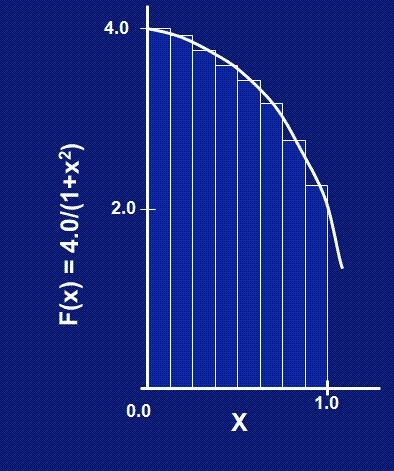
\includegraphics[width=4cm]{./graphics/pi}
    \end{center}
  \end{columns}

  \begin{algorithm}[H]
    \caption{Pseudo Code for Calculating Pi}
    \begin{algorithmic}
        \Function{calculate\_pi}{}
        \State $step \gets 1/n$
        \State $sum \gets 0$
        \Do{$i \gets 0\cdots n$}
        \State $x \gets (i+0.5)*step; sum \gets sum + 4/(1+x^2)$
        \EndDo
        \State $pi \gets sum * step$
        \EndFunction
    \end{algorithmic}
  \end{algorithm}
\end{frame}

\begin{frame}{\small SAXPY}
  \begin{itemize}
    \item SAXPY is a common operation in computations with vector processors included as part of the BLAS routines
    \item[] $y\leftarrow \alpha x + y$
%    \item SAXPY is a combination of scalar multiplication and vector addition
    \item Write a SAXPY code to multiply a vector with a scalar.
  \end{itemize}
  \begin{algorithm}[H]
    \caption{Pseudo Code for SAXPY}
    \begin{algorithmic}
      \Program{saxpy}{}
      \State $n \gets$ some large number
      \State $x(1:n) \gets$ some number say, 1
      \State $y(1:n) \gets$ some other number say, 2
      \State $a \gets$ some other number ,say, 3
      \Do{$i \gets 1\cdots n$}
      \State $y_i \gets y_i + a * x_i$
      \EndDo
      \EndProgram{saxpy}
    \end{algorithmic}
  \end{algorithm}
\end{frame}

\begin{frame}[allowframebreaks]{Matrix Multiplication}
  \begin{itemize}
    \item Most Computational code involve matrix operations such as matrix multiplication.
    \item Consider a matrix {\bf C} which is a product of two matrices {\bf A} and {\bf B}:
    \item[] Element {\it i,j} of {\bf C} is the dot product of the $i^{th}$ row of {\bf A} and $j^{th}$ column of {\bf B}
    \item Write a MATMUL code to multiple two matrices.
  \end{itemize}
  \begin{center}
    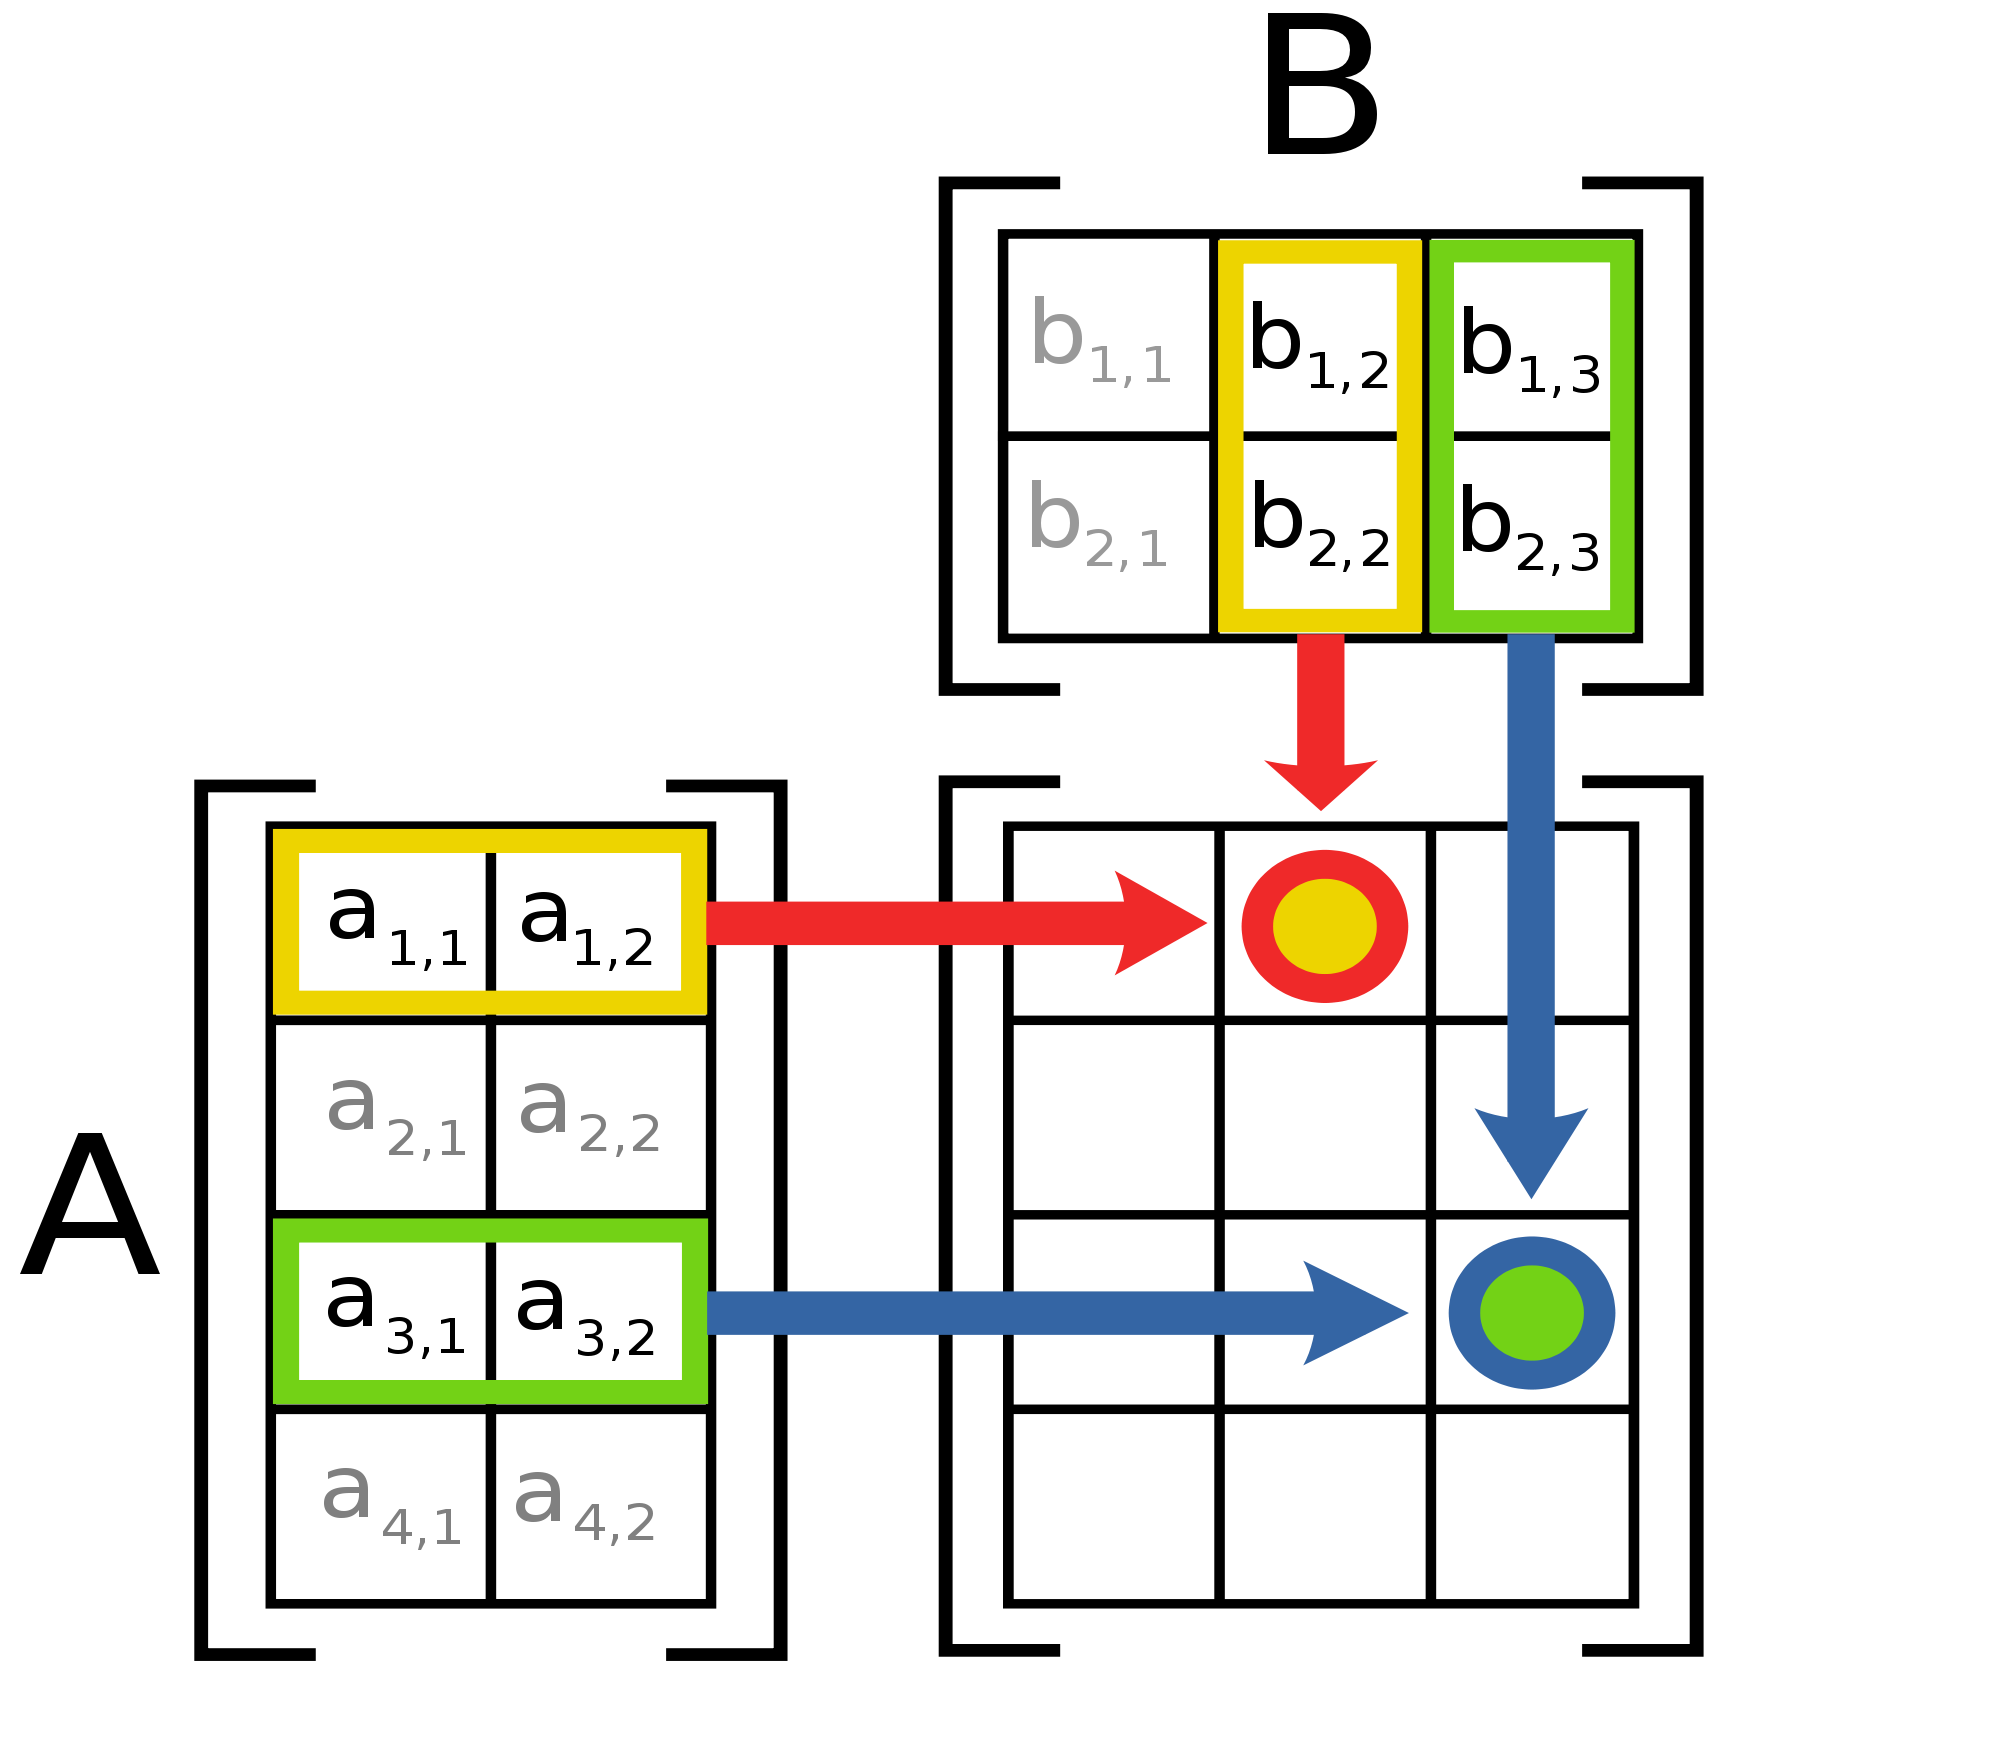
\includegraphics[width=0.3\textwidth]{./graphics/matmul}
  \end{center}

  \begin{algorithm}[H]
    \caption{Pseudo Code for MATMUL}
    \begin{algorithmic}
      \Program{matmul}{}
      \State $m,n \gets$ some\,large\,number $\le 1000$
      \State Define $a_{mn}, b_{nm}, c_{mm}$
      \State $a_{ij} \gets i+j; b_{ij} \gets i-j; c_{ij} \gets 0$
      \Do{$i \gets 1\cdots m$}
      \Do{$j \gets 1\cdots m$}
      \State $c_{i,j} \gets \sum^{n}_{k=1} a_{i,k}*b_{k,j}$
      \EndDo
      \EndDo
      \EndProgram{matmul}
    \end{algorithmic}
  \end{algorithm}
\end{frame}

\end{document}

